% interactapasample.tex
% v1.05 - August 2017

\documentclass[]{interact}

\usepackage{epstopdf}% To incorporate .eps illustrations using PDFLaTeX, etc.
\usepackage[caption=false]{subfig}% Support for small, `sub' figures and tables
%\usepackage[nolists,tablesfirst]{endfloat}% To `separate' figures https://it.overleaf.com/project/5bbc5c481ace70551dd2c703and tables from text if required
%\usepackahttps://it.overleaf.com/project/5bbc5c481ace70551dd2c703ge[doublespacing]{setspace}% To produce a `double spaced' document if required
%\setlength\parindent{24pt}% To increase paragraph indentation when line spacing is doubled
\usepackage{soul}
\usepackage{amsmath,amssymb} 
\usepackage[natbibapa,nodoi]{apacite}% Citation support using apacite.sty. Commands using natbib.sty MUST be deactivated first!
\setlength\bibhang{12pt}% To set the indentation in the list of references using apacite.sty. Commands using natbib.sty MUST be deactivated first!
\renewcommand\bibliographytypesize{\fontsize{10}{12}\selectfont}% To set the list of references in 10 point font using apacite.sty. Commands using natbib.sty MUST be deactivated first!
\theoremstyle{plain}% Theorem-like structures provided by amsthm.sty
\newtheorem{theorem}{Theorem}[section]
\newtheorem{lemma}[theorem]{Lemma}
\newtheorem{corollary}[theorem]{Corollary}
\newtheorem{proposition}[theorem]{Proposition}

\theoremstyle{definition}
\newtheorem{definition}[theorem]{Definition}
\newtheorem{example}[theorem]{Example}

\theoremstyle{remark}
\newtheorem{remark}{Remark}
\newtheorem{notation}{Notation}

\usepackage[pdftex,colorlinks=true,urlcolor=blue,citecolor=black,anchorcolor=black,linkcolor=black]{hyperref}
\usepackage{xcolor}
\newcommand{\mengyi}[1]{\textcolor{blue}{#1}}
\newcommand{\erica}[1]{\textcolor{red}{#1}}

\usepackage{algorithm} 
\usepackage{algorithmic} 
\renewcommand{\algorithmicrequire}{ \textbf{Input:}} %Use Input in the format of Algorithm
\usepackage{soul}
\usepackage{todonotes}

\begin{document}

%\articletype{ARTICLE TEMPLATE}% Specify the article type or omit as appropriate

\title{Mathematical Programming Representation of Discrete-Event Simulation}
\maketitle
\begin{abstract}

\end{abstract}

\section{Introduction}
Discrete Event Simulation (DES) is one of the most used tool for performance evaluation of %discrete event dynamic
complex systems and, hence, simulation--optimization algorithms are widely used %developed for optimizing the parameters of such systems. 
when performance evaluation has to be coupled with optimization, i.e., when the best system configuration, according to some criteria, has to be found meanwhile guaranteeing a given value of some performance measure.  
Most of the state--of--the--art simulation--optimization algorithms consider DES as a \textit{black--box} function, and the structure of DES models has been seldom studied. Under the black--box setting, simulation--optimization algorithms work in an iterative way, alternating simulation and optimization procedures, and always require %huge amount of 
many iterations to explore the %search 
feasible region of the optimization problem, %and can be
thus possibly leading to %computationally inefficient. 
computational inefficiency.
On the contrary, a minority of the simulation--optimization literature explores the structure of the DES models, and %that
such research is referred to as \textit{white--box} simulation--optimization. The benefit of white--box simulation--optimization is the saving of simulation budget due to the fact that %since 
the optimization procedure is guided by the information contained in the structure of the DES model. However, the barrier to the use of white--box simulation--optimization is how to model DES as white--box, so that it eventually favors optimization. This work proposes a procedure to establish a white--box simulation model, which is equivalent Mathematical Programming Representation (MPR), based on the well-known event--scheduling logic for certain types of DES models. 
Specifically, the modeling procedure, the conditions under which it can be applied and some examples are discussed. 

%In this work, we present how to establish an equivalent Mathematical Programming Representation (MPR) of Discrete Event Simulation (DES). The MPR depicts the dynamics of an event-scheduling approach of simulation modeling with a certain sample path. To develop the MPR, state variables, events, initial state, termination condition and the samples of the random variate should be provided. All requirement is also essential each time an event-scheduling algorithm is programmed. Furthermore, the proposed approach is quite routined. Thus, no extra knowledge or skills are required when one has the event-scheduling simulation implementation and wants to apply our approach. Besides the modeling approach, we provide the conditions to check before applying our approach, and discuss what the modifications can be done when some conditions are violated. Some examples are also given.

%Considering the literature on simulation--optimization, 
\cite{chan2008optimization} proposed a modeling framework to translate a DES model into an MPR model in a general sense. Their modeling framework is based on the Event Relationship Graph (ERG) of the system dynamics. To derive the MPR, % model, 
an ERG of the discrete event system has to be constructed and expanded to an elementary ERG (EERG) model, and a routine procedure can be applied to translate the EERG model into an MPR. %model. 
However, this procedure has some limitations. First, deriving an ERG is not an easy task, and the user has to pay quite much attention to detect all the event relationships and complete the triggering conditions between each pair of related events. %That 
The difficulty of developing ERG limits the wide spread of this procedure. 
Second, the modeling procedure is case--by--case, which means the user has to first identify which situations he/she faces by analyzing the EERG, and then choose the appropriate model, including the variables and constraints. This is quite %a burden
difficult, since EERG is an expansion of ERG and the resulting graph could be huge and writing down the complete MPR model could be even impossible.  This work proposes a procedure that does not need % without plotting 
the ERG and %the modeling procedure 
can be used to automatically generate in a general--purpose programming language. Despite %taking different paths
being different, the MPRs proposed in this work and \cite{chan2008optimization} lead to %the 
equivalent results, which, in turn, are both equivalent to a simulation realization.

%When there is already a DES model, 
The benefit of developing an MPR might be not obvious (especially when there is already a DES model) due to the high complexity of solving MPR. 
%One may be confused about the motivation of this work, i.e., why one wants the MPR when he/she has already a simulation model at hand, since the complexity of solving mathematical programming is usually high. 
However, the MPR of a simulation model favors the optimal design and control of the discrete event systems and can use %thanks 
the vast theory and methodological developing in the mathematical programming (MP) field. Many works in the literature show the potentiality of this research direction. For instance, the gradient can be conveniently estimated from the simulation model, if the MPR is approximated into Linear Programming (LP) and %solving 
the dual can be conveniently obtained \citep{chan2008optimization, zhang2020simulation}. Moreover, if some of the parameters in the MPR are changed to decision variables, the MPR becomes an integrated simulation--optimization model. Solving the integrated model provides the optimal solution of the optimization problem \citep{matta2008simulation}. MP--based algorithms, such as linear programming approximation \citep{alfieri2012mathematical}, Benders decomposition \citep{weiss2015buffer}, column generation \citep{alfieri2020time}, have been applied to improve the efficiency of %solving the 
integrated MP model solution. 

The application of MPR--based simulation--optimization approaches is usually found in operations management of manufacturing and service systems. The integrated simulation--optimization model has proved itself to be well suited in solving the buffer allocation problem \citep{zhang2020BAP}. %The most efficient approach to finding the sample--path global optimal of the buffer allocation problem of serial production line is developed based on it \citep{zhang2020BAP}. 
Thanks to the flexibility of DES in evaluating complex systems, the buffer allocation problem of production systems with complex blocking mechanism, such as kanban control, base stock control, extended kanban control, can be managed \citep{pedrielli2015integrated}. Thanks to the flexibility of MPR in modeling optimization problems, problems involving real--valued decision variables such as optimal production rate \citep{tan2015mathematical}, bottleneck detection and throughput improvement problem \citep{zhang2020models} have all been well addressed and the sample--path global optimal solution can be obtained. %It is worthy to notice that, 
Before the above mentioned works were proposed, there were many state--of--the--art heuristic approaches addressing those problems, but without any guarantee of global or local optimality. Thus, the development of MPR--based simulation--optimization has made its contribution in the research area of manufacturing and service system optimization.

%To extend the application of the MPR-based simulation optimization approaches, there is a need of modeling approach to translating DES into MPR under general settings.

The rest of the paper is organized as follows. 

\section{MPR generation procedure}
\subsection{Event-scheduling execution logic of DES } \label{sec:SimAlgo}

The event-scheduling approach is the logic behind all major simulation software and used by practitioners when developing simulation codes with general purpose languages \citep{law2014simulation}. The logic is briefly shown in Figure \ref{Fig:SimAlgo}. The fundamental elements are the system states and the events. The system state is a collection of state variables to describe the system at a particular time. An event execution can lead to the change of system state%, the events of the same type change the system state with the same function
. The event list contains the scheduled but not executed events together with occurring times. When simulation is launched, the system state and the event list is initialized with user-defined values, and the simulation clock is set to zero. The event with the earliest occurring time in the event list will be executed, and the system evolves into a new state together with the simulation clock. The new state may enable to schedule new events, i.e., adding new event together with execution time to the event list, or cancel events, i.e., removing some event executions from the event list. There is usually a delay between time when an event is added to the event list and the time when the event is executed, but the delay might be equal to zero or positive. In the remaining of this work, we refer time when an event is added to the event list as the \textit{scheduling time}. The algorithm will terminate with certain conditions. 

\begin{figure}[h]
	\centering
	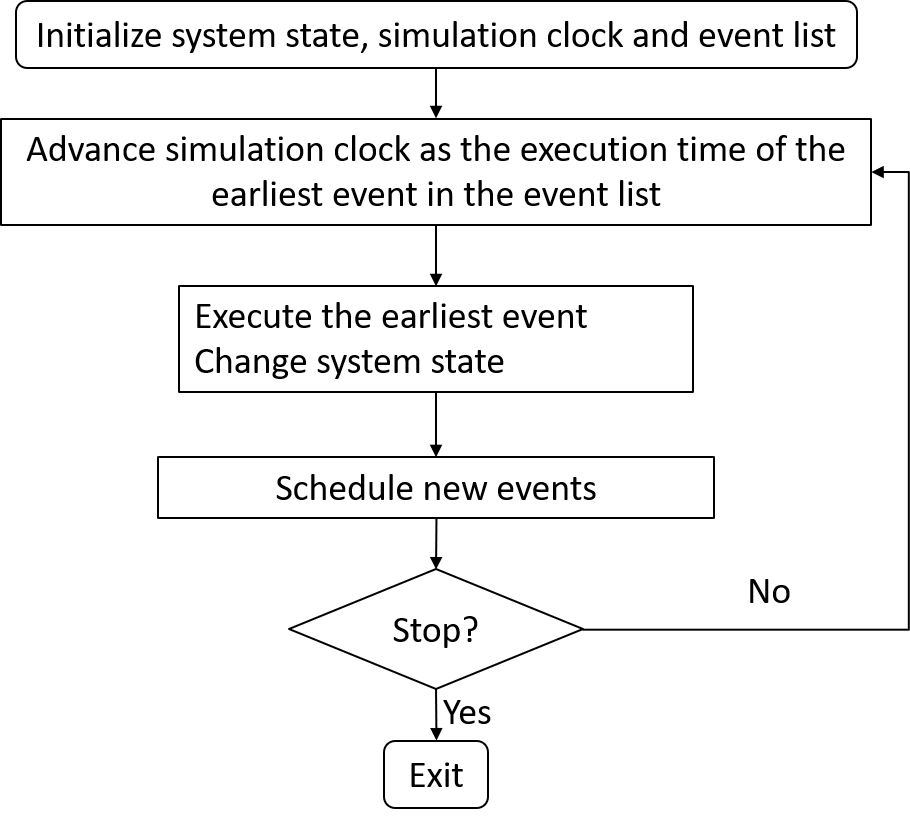
\includegraphics[width=0.6\textwidth]{Figures/EventSimAlgo.png}
	\caption{Event-scheduling simulation algorithm.}
	\label{Fig:SimAlgo}
\end{figure}

%\section{Mathematical programming representation of DES}
In this section, a procedure to translating DES models into MRP is introduced. Before presenting the procedure, the conditions that the DES model has to satisfy in order to have the procedure applicable, are described.

\subsection{Assumptions}

To apply the procedure proposed in this work, the following assumptions must be satisfied.


\begin{enumerate}
	\item State variables are integer.
	\item For all the events $e^{\xi}$ of type $\xi$, the \textit{scheduling conditions} are in the form $a^{\xi}_s\le s \le c^{\xi}_s$ for certain state variable $s$, when multiple state variables are involved, they are combined using logical operator "AND".
	%and combined with logic operator ``AND" when multiple state variables are involved, where $a^{\xi,s}$ and $b^{\xi,s}$ are given.
	%\item The scheduling condition of an event is independent of the history and not changed along time.% (It could be possible to define more state variables in case of history dependence and time-variant scheduling conditions.)
	%\item An event execution of $e^{\xi}$ leads to (integer) increment or decrement equal to $\Delta^{\xi}_s$ of certain state variables $s$, and $\Delta^{\xi}_s$ is not changed along time. (A direct evaluation can be modeled in this way.)
	\item The delay between the scheduling time and the execution time of event $e^{\xi}$ are independent and identically distributed random variables. %(\textit{This point is different from ERG. In ERG, the delay is dependent on the edge, i.e, a couple of events, but I consider delay dependent on a single event.})
	\item When more than one event in the event list have the same execution time% as the earliest execution time
	, the execution sequence is immaterial, i.e., each execution sequence leads to the same new system state and new event list when the simulation clock is advanced.	
	%	the system state, the event list and the number of past executions of each event type are independent of the sequence of execution when the simulation clock is advanced.
	\item Simulation terminates when the number of execution of each event $e^{\xi}$ reaches $N^{\xi}$, which is known, i.e., the number of entities in the system is known. 
	%\item There is no event cancellation.
\end{enumerate}

The first assumption says that the state variables should be integer. Integer variables widely exist in DES models, such as number of jobs in buffers, idle servers, and binary variables to model system behavior and control. A discrete state variable can be translated into an integer variable or a set of binary variables. For real-valued state variables, it can be approximately discretized. Thus, the first assumption is fairly general.

The second condition is, instead, more strict. However, if one model does not satisfy this condition, one can consider to introduce extra binary variables to satisfy assumption (2). For instance, if the condition to schedule event $e^{\xi}$ is $s\le a^{\xi} \ OR\ s\ge b^{\xi}$, a binary variable $\tilde{s}$ is introduced to the model, and $\tilde{s}$ is equal to one if and only if 
$s\le a^{\xi} \ OR\ s\ge b^{\xi}$. 

 As for the third condition, if the delay is not an iid random variate, it should be splitted into several events so that each event has iid delay. For instance, if the distribution of service time depends on the job type, the event of \textit{finishing} a job should be splitted such that the \textit{finishing} of each job type is represented by one event. 
 
The forth condition, in practice, says that the execution time is the only attribute of priority for the event executions in the event list. If one would like to specify the priority to some events having the same execution time, he/she can specify the priority by adding the event with lower priority to the event list after the execution of the event with higher priority, which can be done by introducing extra binary variables.

The fifth condition specifies the termination condition. Specifically, for queueing systems, the termination condition refers to the number of jobs passing through each station. 

%The proposed procedure cannot handling event cancellation, as stated in the last assumption.

\subsection{Mathematical programming model}

The MPR represents the dynamics of the simulated system. Specifically, event scheduling time, event execution time and state variable changes during simulation can all be seen in the MPR as decision variables. The $i$-th scheduling time and the $i$-th execution time of event $e^{\xi}$ are denoted by $e^{\xi,0}_{i}$ and $e^{\xi,1}_{i}$, respectively. The system state changes with a series of event executions,  and $\mathcal{E}_k$ denotes the time of the $k$-th execution. The index $i$ represents the sequence of scheduling or execution of a specific event type, and the index $k$ represents the sequence of execution of general event types. The simulation clock is initialized to zero with $\mathcal{E}_0 = 0$. $e^{\xi,0}_{i}$, $e^{\xi,1}_{i}$ and $\mathcal{E}_k$ are all real-valued. The notation $u^s_k$ is used to denote the value of state variable $s$ just after the $k$-th execution, i.e., just after $\mathcal{E}_k$. The domain of variable $u^s_k$ should be integer. The initial system state is given as $u^s_0$. Some binary variables are also used in the MPR, and they are introduced as the model is explained in details. 


To implement the event-schedule algorithm and generate MPR, for each event type, the conditions to schedule, the conditions to cancel, the distribution of  delay between scheduling and execution and the state variable changes upon execution should be provided. In the event list, multiple executions of the same event type are allowed. For instance, in a G/G/m queue system, when all the servers are occupied, there are $m$ executions of departure event in the event list. The number of executions of event $e^{\xi}$, denoted by $\beta^{\xi}$, is also mandatory to develop the MPR.

The notations of some sets are as follows. The set of all event types is denoted by $\Xi$. $I^{\xi}$ denotes the set of $\{1,...,N^{\xi}\}$, which is the number of executions of event $e^{\xi}$, and $K$ denotes the set of $\{1,...,\sum_{\xi\in\Xi}N^{\xi}\}$, which is the number of executions of all events types. $S$ denotes the set of state variables. $S^{\xi}$ and $S^{\bar{\xi}}$ denote the set of state variables which is relevant to scheduling and cancellation condition of event $e^{\xi}$, respectively.


\subsubsection{Event execution time}
The first group of constraints, denoted by group A, are the constraints binding executions $e^{\xi,1}_i$ and $\mathcal{E}_k$. Binary variables $w^{\xi}_{i,k}$ are used, and $e^{\xi,1}_i$ and $\mathcal{E}_k$ are binded if and only if $w^{\xi}_{i,k}$ is equal to one, as shown in constraints (A1) and (A2). Constraints (A3) and (A4) state that each $e^{\xi,1}_i$ can be binded to one and only one $\mathcal{E}_k$. Constraints (A5) imply that the $\mathcal{E}_{k}$ are temporally sequenced with index $k$. Constraints (A6) show that the $i$-th execution of event $e^{\xi}$ cannot be binded to an execution earlier than $(i-1)$-th execution of event $e^{\xi}$.
%the index executions of the same event type is sequenced along with the index of $\mathcal{E}_k$.

\begin{eqnarray}
e^{\xi,1}_i-\mathcal{E}_k\ge M(w^{\xi}_{i,k}-1) & \forall\ \xi\in\Xi,i\in I^{\xi},k\in K&(A1)\nonumber\\
\mathcal{E}_k-e^{\xi,1}_i\ge M(w^{\xi}_{i,k}-1) & \forall\ \xi\in\Xi,i\in I^{\xi},k\in K&(A2)\nonumber\\
\sum_{k\in K} w^{\xi}_{i,k} =1& \forall\ \xi\in\Xi,i\in I^{\xi}&(A3)\nonumber\\
\sum_{\xi\in \Xi}\sum_{i\in I^{\xi}} w^{\xi}_{i,k} =1&\forall\ k\in K&(A4)\nonumber\\
\mathcal{E}_{k}-\mathcal{E}_{k-1}\ge 0&\forall\ k\in K&(A5)\nonumber\\
\sum_{k\in K} kw^{\xi}_{i,k} - \sum_{k\in K} kw^{\xi}_{i-1,k} \ge 1&  \forall\ \xi\in\Xi,i\in I^{\xi}&(A6)\nonumber
\end{eqnarray}

\subsubsection{Multiple-execution events}
The second group of constraints, denoted by group B, are the constraints binding event scheduling $e^{\xi,0}_i$ and event execution $e^{\xi,1}_{i^{'}}$. If the event is single--execution, i.e., the maximal number of executions in the event list is equal to one, the $i$-th execution $e^{\xi,1}_i$ is binded to the $i$-th scheduling with a delay $t^{\xi}_{i}$, as in constraints (B1), where $t^{\xi}_{i}$ is a sample of delay between scheduling and execution. Thus, the variable $e^{\xi,1}_{i} $ can be replaced by $e^{\xi,0}_{i} + t^{\xi}_{i}$ and the MPR model is reduced.
\begin{eqnarray}
e^{\xi,1}_{i} - e^{\xi,0}_{i} = t^{\xi}_{i} & \forall \xi\in\Xi, i\in I^{\xi}&(B1) \nonumber
\end{eqnarray}

If event $e^{\xi}$ is a multiple-execution event, i.e., the maximal number of executions in the event list $\beta^{\xi}$ is at least two, a late scheduled execution could overtake an early scheduled one, since the delay time between scheduling and execution is a random variate. For instance, in a G/G/m queue, the first starting job may be not the first leaving job, if its service time is pretty long. Thus, the binary variable $y^{\xi}_{i,i^{'}}$ is introduced, and the $i$-th scheduling of event $e^{\xi}$ is the $i^{'}$-th execution when $y^{\xi}_{i,i^{'}}$ is equal to one, as in constraints (B2) and (B3). Constraints (B4) and (B5) show that each $e^{\xi,1}_{i^{'}}$ can be binded to one and only one $e^{\xi,0}_{i}$. Constraints (B6) imply that the $i$-th scheduling cannot be binded to an execution earlier than the $(i+\beta^{\xi})$-th, since at most $\beta^{\xi}$ executions are allowed to be in the list at the same time. For the same reason, constraints (B7) state that $i^{'}$-th execution cannot be binded to the scheduling later than the $(i^{'}-\beta^{\xi})$-th. For instance, in a G/G/2 queue, the third arrival job cannot be the first departure job, since its service starts after the first departure.
\begin{eqnarray}
e^{\xi,1}_{i^{'}} - e^{\xi,0}_{i} \ge t^{\xi}_{i} +M(y^{\xi}_{i,i^{'}}-1) & \forall \xi\in\Xi, i, i ^{'}\in I^{\xi}&(B2)\nonumber\\
e^{\xi,0}_{i} - e^{\xi,1}_{i^{'}}  \ge -t^{\xi}_{i} +M(y^{\xi}_{i,i^{'}}-1) &  \forall \xi\in\Xi, i, i ^{'}\in I^{\xi}&(B3)\nonumber\\
\sum_{i\in I^{\xi}} y^{\xi}_{i,i^{'}} = 1										&  \forall \xi\in\Xi, i ^{'}\in I^{\xi} &(B4)\nonumber\\
\sum_{i^{'}\in I^{\xi}} y^{\xi}_{i,i^{'}} = 1 									& \forall \xi\in\Xi, i \in I^{\xi}&(B5)\nonumber\\
\sum_{i^{'}=i+\beta^{\xi}}^{N^{\xi}} y^{\xi}_{i,i^{'}}=0					&  \forall \xi\in\Xi, 1\le i\le N^{\xi}-\beta^{\xi}&(B6)\nonumber\\
\sum_{i=1}^{i^{'}-\beta^{\xi}} y^{\xi}_{i,i^{'}}=0							& \forall \xi\in\Xi,\ \beta^{\xi}+1\le i^{'} \le N^{\xi}&(B7)\nonumber
\end{eqnarray}



\subsubsection{Constraints for scheduling new events}
The third group of constraints, denoted by group C, state that an execution of event $e^{\xi}$ can be scheduled right after $\mathcal{E}_k$ if the condition for scheduling an event $e^{\xi}$ is true. Binary variables $x^{\xi}_{i,k}$ is used, and $x^{\xi}_{i,k}$ equal to one represents that the $i$-th scheduling of event $e^{\xi}$ is enabled by $\mathcal{E}_k$, as in constraints (C1) and (C2). As stated in Section 3.1, the condition for scheduling event $e^{\xi}$ is a set of inequalities in the form $a^{\xi}_s\le s \le c^{\xi}_s$ combined with operator ``AND". Binary variables $z^{\xi}_{k}$ are used to verify that condition, and if $z^{\xi}_{k}$ is equal to one, the condition is true, as in constraints (C3) and (C4). Moreover, a set of binary variables $v^{\xi,s,0}_k$ and $v^{\xi,s,1}_k$ are used to verify if the condition is false. Specifically, constraints (C5) state that if  $v^{\xi,s,a}_k$ is equal to one, $u^s_k$ will be smaller than $a^{\xi,s}$, and hence, the inequality $a^{\xi}_s\le s$ is violated. Similar for constraints (C6), if $v^{\xi,s,b}_k$ is equal to one, $s \le c^{\xi}_s$ is violated. Constraints (C7) imply that $z^{\xi}_{k}$ is equal to one if and only if $a^{\xi}_s\le s \le c^{\xi}_s$, and that $z^{\xi}_{k}$ is equal to zero if and only if $a^{\xi}_s\le s \le c^{\xi}_s$ is violated. Constraints (C8) state that if the condition to schedule $e^{\xi}$ is true, an execution of $e^{\xi}$ has to be added into the event list. Constraints (C9) show that each scheduling is enabled by one and only one $\mathcal{E}_{k}$. Constraints (C10) show that if the $i$-th scheduling of event $e^{\xi}$ is scheduled by execution $\mathcal{E}_{k}$, the $(i-1)$-th execution cannot be scheduled by an execution later than $\mathcal{E}_{k}$. 
%index of scheduling is sequenced along with the index of event execution $\mathcal{E}_{k}$. 
%Constraints (C11) imply that the $(i+\beta^{\xi},k)$-th scheduling of event $e^{\xi}$ must occur after the $i$-th execution. 

\begin{eqnarray}
e^{\xi,0}_i-\mathcal{E}_{k} \ge M(x^{\xi}_{i,k}-1)& \forall\ \xi\in \Xi,k\in K,i\in I^{\xi}&(C1)\nonumber\\
\mathcal{E}_{k} -e^{\xi,0}_i\ge M(x^{\xi}_{i,k}-1)&\forall\ \xi\in \Xi,k\in K,i\in I^{\xi}&(C2)\nonumber\\
u^s_k - a^{\xi,s} \ge M(z^{\xi}_{k}-1)&\forall\ \xi\in \Xi,k\in K,s\in S&(C3)\nonumber\\
b^{\xi,s} - u^s_k \ge M(z^{\xi}_{k}-1)&\forall\ \xi\in \Xi,k\in K,s\in S&(C4)\nonumber\\
( a^{\xi,s}-1) - u^s_k \ge M(v^{\xi,s,0}_k-1) & \forall\ \xi\in \Xi,k\in K,s\in S &(C5)\nonumber\\
u^s_k -  (b^{\xi,s}+1) \ge M(v^{\xi,s,1}_k-1) & \forall\ \xi\in \Xi,k\in K,s\in S &(C6)\nonumber\\
1 - z^{\xi}_{k} \le \sum_{s\in S^{\xi}} v^{\xi,s,0}_k + \sum_{s\in S^{\xi}} v^{\xi,s,1}_k&\forall\ \xi\in \Xi,k\in K&(C7)\nonumber\\
\sum_{i\in I^{\xi}} x^{\xi}_{i,k} = z^{\xi}_k&\forall\ \xi\in \Xi,k\in K&(C8)\nonumber\\
\sum_{k\in K} x^{\xi}_{i,k} =1& \forall\ \xi\in \Xi,i\in I^{\xi}&(C9)\nonumber\\
\sum_{k\in K} kx^{\xi}_{i,k} - \sum_{k\in K} kx^{\xi}_{i-1,k} \ge 1&  \forall\ \xi\in \Xi,i\in I^{\xi}&(C10)\nonumber\\
\sum_{k\in K} kx^{\xi}_{i+1,k} - \sum_{k\in K} kw^{\xi}_{i,k} \ge 0&  \forall\ \xi\in \Xi,i\in I^{\xi}, t^{\xi} = 0&(C11)\nonumber\\
x^{\xi}_{i,k} = x^{\tilde{\xi}}_{i,k}&  \forall\ \xi\in \Xi,i\in I^{\xi}, t^{\xi} > 0&(C12)\nonumber
\end{eqnarray}

Different rules are applied to zero-delay events and positive-delay events. First, all the zero-delay events are single-execution, because when the delay between scheduling and execution of an event is zero, multiple executions is equivalent to sequential scheduling of a single-execution event. Thus, for zero-delay events, constraints (C11) are relevant, which state that a new event can be scheduled only after the previous execution is conducted. For the event $e^{\xi}$ with strictly positive delay, the following routine should be followed to formulate a correct MPR. A \textit{counting} events ${e}^{\tilde{\xi}}$, which has the same  scheduling condition as $e^{\xi}$ and is zero-delay should be included artificially. The execution of ${e}^{\tilde{\xi}}$ will increment the number of executions of $e^{\xi}$, which is a state variable, by one. Constraints of group A and constraints (B1) (C1), (C2), (C10) and (C11) should also be applied to all counting events. Since each time the condition to schedule $e^{\xi}$ is true, event ${e}^{\tilde{\xi}}$ can also be scheduled, the $i$-th scheduling of event $e^{\xi}$ and ${e}^{\tilde{\xi}}$ should be enabled by the same execution, as stated in constraints (C12), and there is no need to repeat constraints (C3) to (C9) for event ${e}^{\tilde{\xi}}$. In many cases, an event can play the role of counting event for another event, so there is no need to create a duplicating event. For instance, a DES model of G/G/m queue is composed of three events, which are arrival, start and finish. The condition to schedule both start and finish events is an idle server and a job in the queue, and start event is zero-delay and increases the number of busy server by one, which is equivalent to the number executions of finish events. Thus, the start event can be used as the counting event for finish event


%First, multiple execution events should all have positive delay. In fact, when the delay between scheduling and execution of an event is zero, multiple executions is equivalent to sequential scheduling of a single-execution event. For the event $e^{\xi}$ with strictly positive delay, the following routine should be followed to formulate a correct MPR. An event ${e}^{\tilde{\xi}}$ that has the same scheduling condition as $e^{\xi}$ and is zero-delay should be included artificially. The reason to introducing $e^{\tilde{\xi}}$ is not to limit the number of executions, but to allow scheduling of multiple executions, instead, thus ${e}^{\tilde{\xi}}$ is named as the \textit{duplicating} event of event $e^{\xi}$. According to constraints (C9), at most one execution can be scheduled after execution of $\mathcal{E}_{k}$. To schedule multiple executions, the artificial event is used to make sure that the number of executions of event $e^{\xi}$ can reach $\beta^{\xi}$ if the condition to schedule is satisfied. Each time the condition to schedule $e^{\xi}$ is true, event ${e}^{\tilde{\xi}}$ can also be scheduled. Thus, the $i$-th scheduling of event $e^{\xi}$ and ${e}^{\tilde{\xi}}$ should be enabled by the same execution, as stated in constraints (C11), and there is no need to repeat constraints (C3) to (C9) for event ${e}^{\tilde{\xi}}$. In many cases, an event can play the role of duplicating event for another event, so there is no need to create a duplicating event. For instance, a DES model of G/G/m queue is composed of three events, which are arrival, start and finish. The condition to schedule both start and finish events is an idle server and a job in the queue, and start event is zero-delay, and finish event is positive-delay. Thus, the start event can be used as the duplicating event for finish event

\subsubsection{Constraints for event cancellation}
The forth group of constraints, denoted by group D, state that executions of event $e^{\xi}$ in the event list can be canceled right after $\mathcal{E}^k$ if the cancellation condition is true. Similar to constraints (C3) to (C7), constraint (D1) to (D5) show that binary variables $z^{\bar{\xi}}_{k}$ are equal to one if the cancellation condition of $e^{\xi}$ is true right after $\mathcal{E}^k$, where binary variable $z^{\bar{\xi}}_{k}$, $v^{\bar{\xi},s,0}_k$ and $v^{\bar{\xi},s,1}_k$ are the counter part of $z^{\xi}_{k}$, $v^{\xi,s,0}_k$ and $v^{\xi,s,1}_k$, but for event cancellation other than event scheduling. Binary variables $\theta^{\xi}_{i,k}$ are used to represent cancellation an execution. Specifically, $\theta^{\xi}_{i,k}$ is equal to one if and only if the $i$-th execution of event $e^{\xi}$ is canceled after execution $\mathcal{E}_k$. For the $i$-th execution of event $e^{\xi}$, integer variables $k^{\xi,0}_i$ represent the index of execution that scheduled it and $k^{\xi,1}_i$ represent its execution sequence. The definition of $k^{\xi,0}_i$ and $k^{\xi,1}_i$ is shown in constraints (D6) to (D8). The $i$-th execution of event $e^{\xi}$ is canceled after execution $\mathcal{E}_k$ if the cancellation condition is true at a certain time between its scheduling $k^{\xi,0}_i$ and execution $k^{\xi,1}_i$, i.e., there exist $k$ between $k^{\xi,0}_i+1$ and $k^{\xi,1}_i-1$ such that $z^{\bar{\xi}}_{k}$ is equal to one. Binary variables $\theta^{\xi}_{i,k}$ is equal to one if and only if the $i$-th execution of event $e^{\xi}$ is canceled since $z^{\bar{\xi}}_{k}$ is equal to one as in constraints (D9) to (D13), where binary variables $\phi^{\xi,0}_{i,k}$ and $\phi^{\xi,1}_{i,k}$ represent if $k$ is smaller than $k^{\xi,0}_i-1$ or greater than $k^{\xi,1}_i+1$, respectively. Binary variables $\gamma^{\xi}_{i,k}$ equal to one show that the $i$-th execution of event $e^{\xi}$ is actually executed as the $k$-th execution $\mathcal{E}_k$, without cancellation, which is implied with constraints (D14) and (D15).


\begin{eqnarray}
u^s_k - a^{\bar{\xi},s} \ge M(z^{\bar{\xi}}_{k}-1)&\forall\ \xi\in \Xi,k\in K,s\in S^{\bar{\xi}}&(D1)\nonumber\\
b^{\bar{\xi},s} - u^s_k \ge M(z^{\bar{\xi}}_{k}-1)&\forall\ \xi\in \Xi,k\in K,s\in S^{\bar{\xi}}&(D2)\nonumber\\
( a^{\bar{\xi},s}-1) - u^s_k \ge M(v^{\bar{\xi},s,0}_k-1) & \forall\ \xi\in \Xi,k\in K,s\in S^{\bar{\xi}} &(D3)\nonumber\\
u^s_k -  (b^{\bar{\xi},s}+1) \ge M(v^{\bar{\xi},s,1}_k-1) & \forall\ \xi\in \Xi,k\in K,s\in S^{\bar{\xi}} &(D4)\nonumber\\
1 - z^{\bar{\xi}}_{k} \le \sum_{s\in S^{\bar{\xi}}} v^{\bar{\xi},s,0}_k + \sum_{s\in S^{\bar{\xi}}} v^{\bar{\xi},s,1}_k&\forall\ \xi\in \Xi,k\in K&(D5)\nonumber\\
k^{\xi,1}_i = \sum_{k\in K}kw^{\xi}_{k,i}&\forall\ \xi,i&(D6)\nonumber\\
k^{\xi,0}_i \ge k + M(y^{\xi}_{i^{'},i}-1) + M(x^{\xi}_{i^{'},k}-1) & \forall\ \xi\in \Xi,i\in I^{\xi} & (D7)\nonumber\\
k^{\xi,0}_i \le k + M(1-y^{\xi}_{i^{'},i}) + M(1-x^{\xi}_{i^{'},k}) &  \forall\ \xi\in \Xi,i\in I^{\xi}&(D8)\nonumber\\
kz^{\bar{\xi}}_k -k^{\xi,0}_i - 1 \ge M(\theta^{\xi}_{i,k}-1)& \forall\ \xi\in \Xi,i\in I^{\xi}&(D9)\nonumber\\
k^{\xi,1}_i - 1 - kz^{\bar{\xi}}_k \ge M(\theta^{\xi}_{i,k}-1)& \forall\ \xi\in \Xi,i\in I^{\xi},k\in K&(D10)\nonumber\\
k^{\xi,0}_i-1 - kz^{\bar{\xi}}_k \ge M(\phi^{\xi,0}_{i,k}-1)&\forall\ \xi\in \Xi,i\in I^{\xi},k\in K&(D11)\nonumber\\
kz^{\bar{\xi}}_k - k^{\xi,1}_i - 1\ge M(\phi^{\xi,1}_{i,k}-1)&\forall\ \xi\in \Xi,i\in I^{\xi},k\in K&(D12)\nonumber\\
1-\theta^{\xi}_{i,k} \le \phi^{\xi,0}_{i,k} + \phi^{\xi,1}_{i,k}&\forall\ \xi\in \Xi,i\in I^{\xi},k\in K&(D13)\nonumber\\
%k^{\xi^{'},1}_{i^{'}} - k^{\xi,0}_i -1 \ge M(\theta^{\xi}_i-1)\\
%k^{\xi,1}_i - 1 - k^{\xi^{'},1}_{i^{'}} \ge M(\theta^{\xi}_i-1)\\
%k^{\xi,0}_i - k^{\xi^{'},1}_{i^{'}} \ge M(\phi^{\xi,0}_{i,i^{'}}-1)\\
%k^{\xi^{'},1}_{i^{'}}-k^{\xi,1}_i\ge M(\phi^{\xi,1}_{i,i^{'}}-1)\\
%1-\theta^{\xi}_i \le \sum_{i^{'}} (\phi^{\xi,0}_{i,i^{'}}+\phi^{\xi,1}_{i,i^{'}})\\
\gamma^{\xi}_{i,k} \ge w^{\xi}_{i,k} - \sum_{k^{'}\in K}\theta^{\xi}_{i,k^{'}}&\forall\ \xi\in \Xi,i\in I^{\xi},k\in K&(D14)\nonumber\\
w^{\xi}_{i,k} - \sum_{k^{'}\in K}\theta^{\xi}_{i,k^{'}} \ge M(\gamma^{\xi}_{i,k}-1) &\forall\ \xi\in \Xi,i\in I^{\xi},k\in K&(D15)\nonumber
\end{eqnarray}



\subsubsection{Constraints  for  state evolution}
Constraints (E1) represent the evolution of state variables. If the $\mathcal{E}_{k}$ is of event type $\xi$, the state variable $s$ is changed by function $f^{\xi}(u^s_{k-1})$. Constraints (E2) to (E4) show the evolution of the state variable $s^{\xi}$, which counts the number of executions of $e^{\xi}$ in the event list. If $z^{\bar{\xi}}_k$ is equal to one, $s^{\xi}$ is set to zero, as in (E2). Otherwise, it is increased by one if a new execution is added and decreased by one if one execution is conducted.
\begin{eqnarray}
u^{s}_{k} =  \sum_{\xi\in \Xi} \sum_{i\in I^{\xi}} \gamma^{\xi}_{i,k} f^{\xi}(u^s_{k-1})& \forall\ s\in S,k\in K&(E1)\nonumber\\
u^{s^{\xi}}_{k}\le \beta^{\xi}(1-z^{\bar{\xi}}_k) & \forall\ \xi\in\Xi,k\in K&(E2)\nonumber\\
u^{s^{\xi}}_{k}\le u^{s^{\xi}}_{k-1} + z^{\xi}_{k-1} - \sum_{i\in I^{\xi}} \gamma^{\xi}_{i,k} + \beta^{\xi}z^{\bar{\xi}}_k& \forall\ \xi\in\Xi,k\in K&(E3)\nonumber\\
u^{s^{\xi}}_{k}\ge u^{s^{\xi}}_{k-1} + z^{\xi}_{k-1} - \sum_{i\in I^{\xi}} \gamma^{\xi}_{i,k} - \beta^{\xi}z^{\bar{\xi}}_k& \forall\ \xi\in\Xi,k\in K&(E4)\nonumber
\end{eqnarray}

If all the events changes the state variables with a fixed increment or decrement equal to $\Delta^{\xi,s}$, constraints (E1) will be changed to (E5), which are linear constraints, and the MPR is a MILP. 
 \begin{eqnarray}
 u^{s}_{k} = u^s_{k-1} + \sum_{\xi\in \Xi} \sum_{i\in I^{\xi}} \gamma^{\xi}_{i,k} \Delta^{\xi,s}& \forall\ s\in S,k\in K&(E5)\nonumber
 \end{eqnarray}
 
\subsubsection{Objective function}
With the constraints above, there is a unique feasible solution in terms of event occurring times, but the binary variables could be multiple, since there could be more than one simultaneous events. Thus, the definition of objective function is quite flexible. 

\section{Examples}

In this section, several examples are presented. For each example, the necessary information to be provided, and then the derivation of MPR are shown.
%Due to the fact that the procedure can be well coded in a sequence of "automatic" steps, the derivation of the MPR is quite trivial.
\subsection{G/G/1 queue}
The first example is a G/G/1 queue. Table \ref{tab:gg1} shows the events composing the DES model of G/G/1, i.e., the arrival $e^a$, the start of service $e^{r}$ and the finish of service $e^{f}$. The state variables includes the state of server $m$, the number of jobs in the queue $q$. Server state $m$ equal to zero represents that the server is idle, and $m$ equal to one implies that the server is occupied. %The numbers of executions of all the events are not shown in the table, but they are used in the MPR model.
Start event can be used as the counting events of finish event, and state variable $m$ equal to zero or one is equivalent to the number of executions of $e^{f}$ in the event list. Arrival event is positive-delay, a counting event $e^{\tilde{a}}$ and the counter of arrival events in the event list $u^a$ are included. 
If the simulation run includes $N$ jobs, the number of executions of events $e^a$, $e^{\tilde{a}}$, $e^r$, $e^f$ are all equal to $N$, i.e, $I^{a}=I^{\tilde{a}}=I^{r}=I^{f}=\{1,...,N\}$ and $K=\{1,...,4N\}$. 

\begin{table}[h]
	\begin{tabular}{|llllll|}\hline
		Variable&Event & Condition to schedule & Delay&$\beta^{\xi}$& State change\\\hline
		$e^{a}$& Arrival & $u^a\le0$ & $t^a$&1& $q++,u^a--$ \\\hline
		$e^{\tilde{a}}$& Counting arrival & $u^a\le0$ & $0$ &1& $u^a++$ \\\hline
		$e^{r}$& Start 	& $1\le q, m\le 0$ & $0$&1& $m++,q--$ \\\hline
		$e^{f}$& Finish & $1\le q,m\le 0$ & $t^{f}$ &1& $m--$\\\hline
	\end{tabular}
	\caption{Events to simulate G/G/1 system.}
	\label{tab:gg1}
\end{table}

The MPR proposed in this work is as follows: 
\begin{eqnarray}
(A1)-(A6),(B1),(C1),(C2),(C8)-(C10)\nonumber\\
%%%%%%%%%%%%%%%%%%%%%%%%%%%%%%%%%%%%%%%%%%%%%%%%%%%%%%%
z^{a}_{k} = 1-u^{a}_{k} &&\forall k \label{GG1:a1}\\
%%%%%%%%%%%%%%%%%%%%%%%%%%%%%%%%%%%%%%%%%%%%%%%%%%%%%%%
u^q_k \ge z^{r}_{k}&&\forall k \label{GG1:s1}\\
- u^q_k \ge M(v^{r,q,0}_k-1)&&\forall k \label{GG1:s2}\\
-u^m_k \ge M(z^{r}_{k}-1)&&\forall k \label{GG1:s3}\\
u^m_k - 1 \ge M(v^{r,m,0}_k-1)&&\forall k \label{GG1:s4}\\
1 - z^{r}_{k} \le v^{r,q,0}_k +v^{r,m,0}_k&&\forall k \label{GG1:s7}\\
%%%%%%%%%%%%%%%%%%%%%%%%%%%%%%%%%%%%%%%%%%%%%%%%%%%%%%%
z^{f}_{k} = z^{r}_{k}&&\forall k \label{GG1:f1}\\
z^{a}_{k}  = z^{\tilde{a}}_{k} &&\forall k \label{GG1:a2}\\
\sum_{k\in K} kx^{r}_{i+1,k} - \sum_{k\in K} kw^{r}_{i,k} \ge 0&&\forall i\label{GG1:s8}\\
%%%%%%%%%%%%%%%%%%%%%%%%%%%%%%%%%%%%%%%%%%%%%%%%%%%%%%%
u^{a}_k = u^{a}_{k-1} - \sum_{i}w^{a}_{i,k} + \sum_{i} w^{\tilde{a}}_{i,k} &&\forall k \label{GG1:E1}\\
u^{m}_k = u^{m}_{k-1} -  \sum_{i}w^{f}_{i,k} + \sum_{i} w^{r}_{i,k} &&\forall k \label{GG1:E4}\\
u^{q}_k = u^{q}_{k-1} +  \sum_{i}w^{a}_{i,k} -  \sum_{i}w^{r}_{i,k}&&\forall k \label{GG1:E5}\\
%%%%%%%%%%%%%%%%%%%%%%%%%%%%%%%%%%%%%%%%%%%%%%%%%%%%%%%%
\mathcal{E}_0 = 0, u^q_0=u^m_0=0\nonumber\\
u^{a}_{k}\in\{0,1\},\ m\in\{0,1\},\ q\in \mathbb{N}
\end{eqnarray}

Group-A constraints are the same as presented in section XXX. All the events are single-execution, so constraints (B1) is applied, and $e^{\xi}_{i,1}$ can be replaced by $e^{\xi}_{i,0}+t^{\xi}_i$ for all event types. For group (C) constraints, (C1), (C2) and (C8) to (C10) are the same as presented in Section XXX. Constraints (C3) to (C7) are expanded. For the arrival events, the scheduling condition is that the execution in the event list is less than one, as in constraints \eqref{GG1:a1}. For the start event, condition $1\le q$ is verified with constraints \eqref{GG1:s1} and \eqref{GG1:s2}, and condition $ m\le 0$ is verified with constraints \eqref{GG1:s3} and \eqref{GG1:s4}. Constraints \eqref{GG1:s7} guarantee that a start event must be scheduled once the scheduling condition is true. Start event can be used as the counting events of finish event, and state variable $m$ is equivalent to the number of executions of $e^{f}$ in the event list, so constraints \eqref{GG1:f1} are included. Arrival event is positive-delay, a counting event $e^{\tilde{a}}$, the counter of arrival events in the event list $u^a$ and constraints \eqref{GG1:a2} are included. Start events is zero-delay, so constraints \eqref{GG1:s8} are applied. Constraints \eqref{GG1:E1} to \eqref{GG1:E5} show the state variable evolution. The objective function of the model is missing, because it can be arbitrary as stated above.

The MPR model proposed in \cite{chan2008optimization} is as follows:
\begin{eqnarray}
\min\{\sum_{i=1}^N (e^{a}_{i,1}+e^{r}_{i,1}+e^{f}_{i,1})\}\nonumber\\
e^{a}_{i,1} - e^{a}_{i-1,1} = t^{a}_{i}&&\forall\ i \label{GG1erg:1}\\
e^{f}_{i,1} - e^{r}_{i,1} = t^{f}_{i}&&\forall\ i\label{GG1erg:2}\\
e^{r}_{i,1} - e^{a}_{i,1} \ge 0&&\forall\ i\label{GG1erg:3}\\
e^{r}_{i,1} - e^{f}_{i-1,1} \ge 0&&\forall\ i\label{GG1erg:4}
\end{eqnarray}

To explain the MPR model, the ERG of G/G/1 queue is first shown in Figure \ref{fig:ERG_GG1}. Each triggering relationship in the ERG, i.e., two connected nodes is represented by one constraint. Constraints \eqref{GG1erg:1} to \eqref{GG1erg:4} state the relationships of $e^a \rightarrow e^a$, $e^s\rightarrow e^f$, $e^a\rightarrow e^s$ and $e^f\rightarrow e^s$, respectively. The objective function is the sum of all the event execution time. As can be seen, the model is a linear programming. 

\begin{figure}[h]
	\centering
	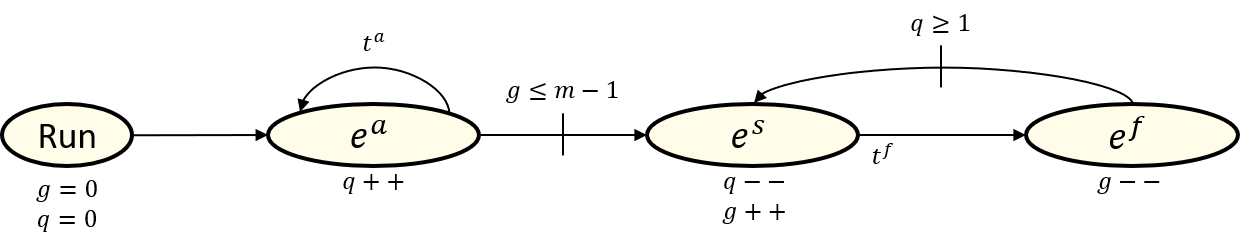
\includegraphics[width=0.6\textwidth]{Figures/ERG_GG1.png}
	\caption{ERG of G/G/1 queue.}
	\label{fig:ERG_GG1}
\end{figure}

\subsection{Single server merge}

A queueing system composed of three servers within a merge architecture is presented in this section. Jobs enter the system at server 1 or server 2, and the buffer in front of the two servers has infinite capacity. It is assumed that all the jobs arrive at time zero. After processing a job, server 1 or 2 can release the job to the finite buffer in front of server 3, if the buffer is not full. The blocking policy is block-after-service. If there is only one space available in the buffer, and both servers 1 and 2 are holding a finished job, server 1 has higher priority to release. After processing a job, server 3 releases the job from the system immediately. 

\begin{figure}[h]
	\centering
	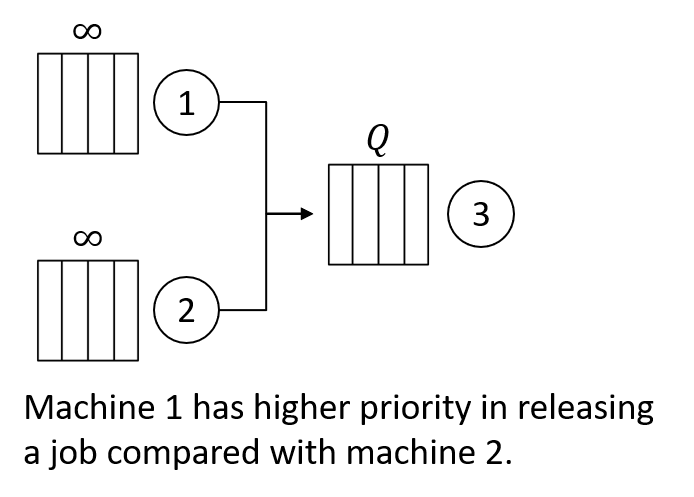
\includegraphics[width=0.4\textwidth]{Figures/merge.png}
	\caption{Example: single server merge.}
\end{figure}

State variables have to be defined in the first place. Variable $m^i$ and $q$ represents the state of server $i$ and the available space in buffer 3, respectively. Both server 1 and 2 have three states, namely \textit{idle}, \textit{working} and \textit{holding a finished job}, and each state refers to $m^i$ equal to $0$, $1$ and $2$ respectively. Server 3 has only two states, \textit{idle} and \textit{working}, and refers to $m^3$ equal to $0$ and $1$, respectively. The servers are initially idle, and buffer 3 is empty, i.e., $m^1=m^2=m^3=0$ and $q=Q$, where $Q$ denotes the capacity of buffer 3.

The events composed the DES model are then defined as in Table \ref{tab:merge}. Event $e^{r,1}$ represents the starting of service of server 1, the scheduling of such event is enabled if server 1 is idle, i.e., $m^1\le 0$. Executing $e^{r,1}$ will increase state variable $m^1$ from 0 to 1. Event $e^{f,1}$ represents the finishing of server 1, scheduling of it requires that server 1 is idle. The delay between scheduling and execution is random variate $t^1$, which is the service time. Executing $e^{f,1}$ makes the server hold a finished job and hence increase state variable $m^1$ from 1 to 2. Events $e^{r,2}$ and $e^{f,2}$ are similar to events $e^{r,1}$ and $e^{f,1}$. The departure events of server 1 and server 2 differ from each other. As long as there is a space available in buffer 3 and server 1 holds a finished job, a departure event of server 1 $e^{d,1}$ can be scheduled. For the departure event of server 2 $e^{d,2}$, one more condition to verify is that server 1 does not hold a finished job due to the priority rule. The execution of departure event of server 1 or 2 will occupy an available space in buffer 3, and make the server idle. The start event of server 3 $e^{r,3}$ is enabled if it is idle and there is at least one job waiting in buffer 3. After execution of $e^{r,3}$, the server becomes busy and the available space in buffer 3 is increased by one. The departure event $e^{d,3}$ can be scheduled if server 3 is working with delay $t^3$, which is a random variate representing the service time of server 3. Execution of  $e^{d,3}$ makes server 3 idle. Since all the stations are composed of a single server, all events are single-execution. 

\begin{table}[h]
	\begin{tabular}{|llllll|}\hline
		Variable&Event & Condition to schedule & Delay&$\beta^{\xi}$& State change\\\hline
		$e^{r,1}$&Start m1 	& $m^1\le 0$ & $0$&1& $m^1++$ \\\hline
		$e^{f,1}$&Finish m1 & $m^1\le 0$ 	& $t^1$ &1& $m^1++$\\\hline
		$e^{d,1}$&Depart m1& $m^1\ge2\ \&\  q\ge 1$&$0$ &1 & $m^1 = m^1-2,\ q--$\\\hline
		$e^{r,2}$&Start m2 	& $m^2\le 0$ & $0$ &1& $m^2++$ \\	\hline
		$e^{f,2}$&Finish m2 & $m^2\le 0$ 	& $t^2$ &1 & $m^2++$\\\hline
		$e^{d,2}$&Depart m2& $m^2\ge2\ \&\ q\ge 1\&$&$0$  &1& $m^2=m^2-2,\ q--$\\
		&&$\ m^1\le 1 $ & &&\\\hline
		$e^{r,3}$& Start m3 & $m^3 \le 0\ \&\ q\le Q-1$&$0$  &1& $m^3++,\ q++$\\\hline
		$e^{d,3}$& Depart m3 & $m^3 \le 0\ \&\ q\le Q-1$ & $t^3$  &1& $m^3--$\\\hline
	\end{tabular}
	\caption{Events to simulate a merge queueing system.}
	\label{tab:merge}
\end{table}

The MPR proposed in this work is as follows: 
\begin{eqnarray}
(A1)-(A6),(B1),(C1),(C2),(C8)-(C10)\nonumber\\
%%%%%%%%%%%%%%%%%   \xi=(s,1)   %%%%%%%%%%%%%%%%%%%%%%%%%%%
- u^{m^1}_k \ge 2(z^{r,1}_{k}-1)&& \forall\ k\label{merge:s1.1}\\
u^{m^1}_k - 1 \ge v^{(r,1),m^1,1}_k-1 && \forall\ k \label{merge:s1.2}\\
1 - z^{r,1}_{k} \le v^{(r,1),m^1,1}_k&&\forall\ k\label{merge:s1.3}\\
z^{f,1}_{k} = z^{r,1}_{k}&&\forall\ k\label{merge:f1.1}\\
%%%%%%%%%%%%%%%%%%   \xi=(s,2)   %%%%%%%%%%%%%%%%%%%%%%%%%%%%%%%%
- u^{m^2}_k \ge 2(z^{r,2}_{k}-1)&& \forall\ k\label{merge:s2.1}\\
u^{m^2}_k - 1 \ge v^{(r,2),m^2,1}_k-1 && \forall\ k \label{merge:s2.2}\\
1 - z^{r,2}_{k} \le v^{(r,2),m^2,1}_k&&\forall\ k\label{merge:s2.3}\\
z^{f,2}_{k} = z^{r,2}_{k} &&\label{merge:f2.1}
\end{eqnarray}
\begin{eqnarray}
%%%%%%%%%%%%%%%%%%%%%%   \xi=(d,1)   %%%%%%%%%%%%%%%%%%%%%%%%%%%%
u^{m^1}_k - 2 \ge 2(z^{d,1}_{k}-1)&& \forall\ k\label{merge:d1.1}\\
1 - u^{m^1}_k \ge v^{(d,1),m^1,0}_k-1 && \forall\ k \label{merge:d1.2}\\
u^{q}_k - 1 \ge z^{d,1}_{k}-1 && \forall\ k\label{merge:d1.3}\\
- u^q_k \ge Q(v^{(d,1),q,0}_k-1) && \forall\ k \label{merge:d1.4}\\
1 - z^{d,1}_{k} \le v^{(d,1),m^1,0}_k + v^{(d,1),q,0}_k&&\forall\ k\label{merge:d1.5}\\
%%%%%%%%%%%%%%%%%%%%%%   \xi=(d,2)   %%%%%%%%%%%%%%%%%%%%%%%%%%%%
u^{m^2}_k - 2 \ge 2(z^{d,2}_{k}-1)&& \forall\ k\label{merge:d2.1}\\
1 - u^{m^2}_k \ge v^{(d,2),m^2,0}_k-1 && \forall\ k \label{merge:d2.2}\\
u^{q}_k - 1 \ge z^{d,2}_{k}-1 && \forall\ k\label{merge:d2.3}\\
- u^q_k \ge Q(v^{(d,2),q,0}_k-1) && \forall\ k \label{merge:d2.4}\\
1 - u^{m^1}_k \ge z^{d,2}_{k}-1&& \forall\ k\label{merge:d2.5}\\
u^{m^1}_k -  2 \ge 2(v^{(d,2),m^1,1}_k-1) && \forall\ k \label{merge:d2.6}\\
1 - z^{d,2}_{k} \le v^{(d,2),m^2,0}_k + v^{(d,2),q,0}_k + v^{(d,2),m^1,1}_k&&\forall\ k\label{merge:d2.7}\\
%%%%%%%%%%%%%%%%%%%%%%   \xi=(s,3)   %%%%%%%%%%%%%%%%%%%%%%%%%%%%
- u^{m^3}_k \ge z^{r,3}_{k}-1&& \forall\ k\label{merge:s3.1}\\
u^{m^3}_k - 1 \ge v^{(r,3),m^3,1}_k-1 && \forall\ k \label{merge:s3.2}\\
Q-1 - u^q_k \ge z^{r,3}_{k}-1&& \forall\ k\label{merge:s3.3}\\
u^q_k - Q \ge Q(v^{(r,3),q,1}_k-1) && \forall\ k\label{merge:s3.4}\\
1 - z^{r,3}_{k} \le v^{(r,3),m^3,1}_k + v^{(r,3),q,1}_k&&\forall\ k\label{merge:s3.5}\\
z^{d,3}_{k} = z^{r,3}_{k}&&\forall\ k\label{merge:d3.1}\\
%%%%%%%%%%%%%%%%%%%%%%%%%%%%%%%%%%%%%%%%%%%%%%%%%%
\sum_{k} kx^{\xi}_{i+1,k} - \sum_{k} kw^{\xi}_{i,k} \ge 0\nonumber\\
\forall \xi\in\{(s,1),(s,2),(s,3),(d,1),(d,2)\}, \forall\ i\label{merge:C11}\\
%%%%%%%%%%%%%%%%%%%%%%   \xi=(d,3)   %%%%%%%%%%%%%%%%%%%%%%%%%%%%
u^{m^1}_k = u^{m^1}_{k-1} + \sum_{i}w^{r,1}_{i,k} + \sum_{i}w^{f,1}_{i,k}  - 2\sum_{i}w^{d,1}_{i,k} &&\forall\ k\label{merge:E1}\\
u^{m^2}_k = u^{m^2}_{k-1} +\sum_{i} w^{r,2}_{i,k}  + \sum_{i}w^{f,2}_{i,k}  - 2\sum_{i}w^{d,2}_{i,k}  &&\forall\ k\label{merge:E2}\\
u^{m^3}_k = u^{m^3}_{k-1} + \sum_{i}w^{r,3}_{i,k}  -  \sum_{i}w^{d,3}_{i,k}  &&\forall\ k\label{merge:E3}\\
u^q_k = u^{q}_{k-1} - \sum_{i}w^{d,1}_{i,k}  -\sum_{i}w^{d,2}_{i,k}  +\sum_{i} w^{r,3}_{i,k}   &&\forall\ k\label{merge:E4}\\
%%%%%%%%%%%%%%%%%%%%%%%%%%%%%%%%%%%%%%%%%%%%%%%%%%%%%%%%
\mathcal{E}_0 = 0, u^{m^1}_0=u^{m^2}_0=u^{m^3}_0=0, u^q_0=Q\nonumber\\
u^{m^1}_k,\ u^{m^2}_k\in\{0,1,2\},\ u^{m^3}_k\in\{0,1\},\ q\in \{0,...,Q\}&& \forall\ k
\end{eqnarray}

If the simulation run includes $N_1$ jobs from server 1 and $N_2$ jobs from server 2, the number of executions of events $e^{r,1}$, $e^{f,1}$, $e^{d,1}$ are equal to $N_1$, the number of executions of events $e^{r,2}$, $e^{f,2}$, $e^{d,2}$ are equal to $N_2$, the number of executions of events $e^{r,3}$, $e^{d,3}$ are equal to $N_1+N_2$, and total number of executions is equal to $5N_1+5N_2$. Group-A constraints are the same as presented in section XXX. All the events are single-execution, so constraints (B1) is applied, and $e^{\xi}_{i,1}$ can be replaced by $e^{\xi}_{i,0}+t^{\xi}_i$ for all event types. For group (C) constraints, (C1), (C2) and (C8) to (C10) are the same as presented in Section XXX. Constraints (C3) to (C7) are expanded as follows. For event $e^{r,1}$, the condition on $m^1$ is verified with constraints \eqref{merge:s1.1} to \eqref{merge:s1.3}. Event $e^{r,1}$ is also a counting event of $e^{f,1}$, so constraints \eqref{merge:f1.1} are included for scheduling $e^{f,1}$. The same constraints are applied to events $e^{r,2}$ and $e^{f,2}$, with constraints \eqref{merge:s2.1} to \eqref{merge:f2.1}. The scheduling conditions of event $e^{d,1}$ and $e^{d,2}$ are verified with constraints \eqref{merge:d1.1} to \eqref{merge:d1.5} and constraints \eqref{merge:d2.1} to \eqref{merge:d2.7}, respectively. For event $e^{r,3}$, the scheduling condition is verified with constraints \eqref{merge:s3.1} ro \eqref{merge:s3.5}. Event $e^{r,3}$ is also a counting event of $e^{d,3}$, so constraints \eqref{merge:d3.1} are included for scheduling $e^{d,3}$. For all the zero-delay events, constraints \eqref{merge:C11} are relevant. Constraints \eqref{merge:E1} to \eqref{merge:E4} state the state variable evolution.

The MPR model proposed in \cite{chan2008optimization} is as follows:

\begin{eqnarray}
\min\{\sum_{i=1}^{N_1} (e^{s,1}_i+e^{f,1}_{i}+e^{d,1}_{i})+\sum_{i=1}^{N_2}(e^{s,2}_i+e^{f,2}_{i}+e^{d,2}_{i}) + \sum_{i}^{} e^{d,2,1}_{i}+\nonumber\\
\sum_{i=1}^{N_1+N_2}(e^{s,3}_i+e^{d,3}_{i}-e^{w:(d,1),(d,2)}_i) +\sum_{i=1}^{N_1+N_2}\sum_{k=1}^{N_1} e^{p:(d,1),(d,2)}_{i,k,i-k}\}\nonumber\\
e^{s,1}_i - e^{d,1}_{i-1} = 0\label{MergeErg:1} \\
e^{f,1}_{i} - e^{s,1}_{i} = t^{1}_i\\
e^{s,2}_i - e^{d,2}_{i-1} = 0\\
e^{f,2}_{i} - e^{s,2}_{i} = t^{2}_i\\
%e^{d,2,1}_{i} - e^{f,2}_{i} \ge 0\\
e^{d,3}_{i} - e^{s,3}_{i} = t^{3}_i\\
e^{d,1}_{i} - e^{f,1}_{i} \ge 0\label{MergeErg:6} \\
e^{s,3}_{i} - e^{d,3}_{i-1} \ge 0\label{MergeErg:7} 
\end{eqnarray}


%%%%%%%%%%%%%%%% e^{d,2,1}_j -> e^{d,2}_i   【Case D】 %%%%%%%%%%%%%%%%%%%%%%%%%%%%%%%%%%%
\begin{eqnarray}
e^{d,2}_i-e^{d,2,1}_j\ge M(\sigma_{(d,2,1):j,(d,2):i}-1)\label{MergeErg:8.1}\\
e^{d,2}_i-e^{d,2,1}_j\ge m(1 - \sigma_{(d,2,1):j,(d,2):i})\\
e^{d,2,1}_{j} \ge e^{d,1}_{k} - M(1-\zeta_{(d,1):k,(d,2,1):j})\\ 
e^{d,1}_{k} \ge e^{d,2,1}_{j} + m\zeta_{(d,1):k,(d,2,1):j} +(1-\zeta_{(d,1):k,(d,2,1):j})\varepsilon\\ 
e^{f,1}_{k+1} \ge e^{d,2,1}_{j} - M(1-\eta_{(d,2,1):j,(f,1):k+1})\\
e^{d,2,1}_{j} \ge e^{f,1}_{k+1} + m\eta_{(d,2,1):j,(f,1):k+1}\\
\gamma_{(d,1):k,(d,2,1):j} - (\zeta_{(d,1):k,(d,2,1):j} + \eta_{(d,2,1):j,(f,1):k+1})+1\ge 0\\
2\gamma_{(d,1):k,(d,2,1):j}-(\zeta_{(d,1):k,(d,2,1):j} + \eta_{(d,2,1):j,(f,1):k+1})\le 0\\
\sum_k\gamma_{(d,1):k,(d,2,1):j}-\sum_i \sigma_{(d,2,1):j,(d,2):i} \ge 0\\
n\sum_{i}\sigma_{(d,2,1):j,(d,2):i} - \sum_k\gamma_{(d,1):k,(d,2,1):j}\ge 0\\
\sum_{i}\sigma_{(d,2,1):j,(d,2):i}\le 1\\
\sum_{j}\sigma_{(d,2,1):j,(d,2):i}\le 1\\
\sum_{j=i}^{n}\sigma_{(d,2,1):j,(d,2):i}\ge \sum_{j=i+1}^{n}\sigma_{(d,2,1):j,(d,2):i+1}\\
\sum_{p=j+1}^n\sum_{q=1}^{i-1} \sigma_{(d,2,1):p,(d,2):q} \ge min\{i-1,n-j\}(1-\sigma_{(d,2,1):j,(d,2):i})\label{MergeErg:8.2}
\end{eqnarray}


%%%%%%%%%%%%%%%% e^{d,3}_j -> e^{d,2,1}_i   【Case D】 %%%%%%%%%%%%%%%%%%%%%%%%%%%%%%%%%%%
\begin{eqnarray}
e^{d,2,1}_i-e^{s,3}_j\ge M(\sigma_{(s,3):j,(d,2,1):i}-1)\label{MergeErg:9.1}\\
e^{d,2,1}_i-e^{s,3}_j\ge m(1 - \sigma_{(s,3):j,(d,2,1):i})\\
e^{s,3}_{j} \ge e^{f,2}_{k} - M(1-\zeta_{(f,2):k,(s,3):j})\\ 
e^{f,2}_{k} \ge e^{s,3}_{j} + m\zeta_{(f,2):k,(s,3):j} +(1-\zeta_{(f,2):k,(s,3):j})\varepsilon\\ 
e^{d,2}_{k+1} \ge e^{s,3}_{j} - M(1-\eta_{(s,3):j,(d,2):k+1})\\
e^{s,3}_{j} \ge e^{d,2}_{k+1} + m\eta_{(s,3):j,(d,2):k+1}\\
\gamma_{(f,2):k,(s,3):j} - (\zeta_{(f,2):k,(s,3):j} + \eta_{(s,3):j,(d,2):k+1})+1\ge 0\\
2\gamma_{(f,2):k,(s,3):j}-(\zeta_{(f,2):k,(s,3):j} + \eta_{(s,3):j,(d,2):k+1})\le 0\\
\sum_k\gamma_{(f,2):k,(s,3):j}-\sum_i \sigma_{(s,3):j,(d,2,1):i} \ge 0\\
n\sum_{i}\sigma_{(s,3):j,(d,2,1):i} - \sum_k\gamma_{(f,2):k,(s,3):j}\ge 0\\
\sum_{i}\sigma_{(s,3):j,(d,2,1):i}\le 1\\
\sum_{j}\sigma_{(s,3):j,(d,2,1):i}\le 1\\
\sum_{j=i}^{n}\sigma_{(s,3):j,(d,2,1):i}\ge \sum_{j=i+1}^{n}\sigma_{(s,3):j,(d,2,1):i+1}\\
\sum_{p=j+1}^n\sum_{q=1}^{i-1} \sigma_{(s,3):p,(d,2,1):q} \ge min\{i-1,n-j\}(1-\sigma_{(s,3):j,(d,2,1):i})\label{MergeErg:9.2}
\end{eqnarray}


%%%%%%%%%%%%%%%% 【Convolution】  e^{d,1} & e^{d,2} %%%%%%%%%%%%%%%%%%%%%%%%%%%%%%%%%%%
\begin{eqnarray}
e^{w:(d,1),(d,2)}_i\le e^{p:(d,1),(d,2)}_{i,k,i-k}\label{MergeErg:10.1}\\
e^{d,1}_k\ge e^{d,2}_{i-k} - M(1-\alpha^{(d,1),(d,2)}_{i,k,i-k})\\
e^{d,2}_{i-k} \ge e^{d,1}_{i-k} + m\alpha^{(d,1),(d,2)}_{i,k,i-k}+(1-\alpha^{(d,1),(d,2)}_{i,k,i-k})\varepsilon\\
e^{p:(d,1),(d,2)}_{i,k,i-k}\ge e^{d,1}_k - M(1-\alpha^{(d,1),(d,2)}_{i,k,i-k})\\
e^{d,1}_k\ge e^{p:(d,1),(d,2)}_{i,k,i-k}+m(1-\alpha^{(d,1),(d,2)}_{i,k,i-k})\\
e^{p:(d,1),(d,2)}_{i,k,i-k}\ge e^{d,2}_k - M\alpha^{(d,1),(d,2)}_{i,k,i-k}\\
e^{d,2}_k\ge e^{p:(d,1),(d,2)}_{i,k,i-k}+m\alpha^{(d,1),(d,2)}_{i,k,i-k}\label{MergeErg:10.2}
\end{eqnarray}


%%%%%%%%%%%%%%%% e^{f,2}_j -> e^{d,2,1}_i   【Case (h)】 %%%%%%%%%%%%%%%%%%%%%%%%%%%%%%%%%%%
\begin{eqnarray}
e^{d,2,1}_i-e^{f,2}_j\ge M(\sigma_{(f,2):j,(d,2,1):i}-1)\label{MergeErg:11.1}\\
e^{d,2,1}_i-e^{f,2}_j\ge m(1 - \sigma_{(f,2):j,(d,2,1):i})\\
e^{f,2}_{j} \ge e^{s,3}_{k} - M(1-\zeta_{(s,3):k,(f,2):j})\\ 
e^{s,3}_{k} \ge e^{f,2}_{j} + m\zeta_{(s,3):k,(f,2):j} +(1-\zeta_{(s,3):k,(f,2):j})\varepsilon\\ 
e^{w:(d,1),(d,2)}_{k+Q} \ge e^{f,2}_{j} - M(1-\eta_{(f,2):j,(w:(d,1),(d,2)):k+Q})\\
e^{f,2}_{j} \ge e^{w:(d,1),(d,2)}_{k+Q} + m\eta_{(f,2):j,(w:(d,1),(d,2)):k+Q}\\
\gamma_{(s,3):k,(f,2):j} - (\zeta_{(s,3):k,(f,2):j} + \eta_{(f,2):j,(w:(d,1),(d,2)):k+Q})+1\ge 0\\
2\gamma_{(s,3):k,(f,2):j}-(\zeta_{(s,3):k,(f,2):j} + \eta_{(f,2):j,(w:(d,1),(d,2)):k+Q})\le 0\\
\sum_k\gamma_{(s,3):k,(f,2):j}-\sum_i \sigma_{(f,2):j,(d,2,1):i} \ge 0\\
n\sum_{i}\sigma_{(f,2):j,(d,2,1):i} - \sum_k\gamma_{(s,3):k,(f,2):j}\ge 0\\
\sum_{i}\sigma_{(f,2):j,(d,2,1):i}\le 1\\
\sum_{j}\sigma_{(f,2):j,(d,2,1):i}\le 1\\
\sum_{j=i}^{n}\sigma_{(f,2):j,(d,2,1):i}\ge \sum_{j=i+1}^{n}\sigma_{(f,2):j,(d,2,1):i+1}\\
\sum_{p=j+1}^n\sum_{q=1}^{i-1} \sigma_{(f,2):p,(d,2,1):q} \ge min\{i-1,n-j\}(1-\sigma_{(f,2):j,(d,2,1):i})\label{MergeErg:11.2}
\end{eqnarray}

%%%%%%%%%%%%%%%% e^{d,3}_j -> e^{s,3}_i   【Case (f)】 %%%%%%%%%%%%%%%%%%%%%%%%%%%%%%%%%%%
\begin{eqnarray}
e^{s,3}_i \ge e^{w:(d,1),(d,2)}_{i}\label{MergeErg:12}
\end{eqnarray}

\begin{eqnarray}
%%%%%%%%%%%%%%%% e^{f,1}_j -> e^{d,1}_i   【Case (f)】 %%%%%%%%%%%%%%%%%%%%%%%%%%%%%%%%%%%
e^{d,1}_i-e^{f,1}_j\ge M(\sigma_{(f,1):j,(d,1):i}-1)\label{MergeErg:13.1}\\
e^{d,1}_i-e^{f,1}_j\ge m(1 - \sigma_{(f,1):j,(d,1):i})\\
e^{f,1}_{j} \ge e^{s,3}_{k} - M(1-\zeta_{(s,3):k,(f,1):j})\\ 
e^{s,3}_{k} \ge e^{f,1}_{j} + m\zeta_{(s,3):k,(f,1):j} +(1-\zeta_{(s,3):k,(f,1):j})\varepsilon\\ 
e^{d,2}_{k+Q} \ge e^{f,1}_{j} - M(1-\eta_{(f,1):j,(d,2):k+Q})\\
e^{f,1}_{j} \ge e^{d,2}_{k+Q} + m\eta_{(f,1):j,(d,2):k+Q}\\
\gamma_{(s,3):k,(f,1):j} - (\zeta_{(s,3):k,(f,1):j} + \eta_{(f,1):j,(d,2):k+Q})+1\ge 0\\
2\gamma_{(s,3):k,(f,1):j}-(\zeta_{(s,3):k,(f,1):j} + \eta_{(f,1):j,(d,2):k+Q})\le 0\\
\sum_k\gamma_{(s,3):k,(f,1):j}-\sum_i \sigma_{(f,1):j,(d,1):i} \ge 0\\
n\sum_{i}\sigma_{(f,1):j,(d,1):i} - \sum_k\gamma_{(s,3):k,(f,1):j}\ge 0\\
\sum_{i}\sigma_{(f,1):j,(d,1):i}\le 1\\
\sum_{j}\sigma_{(f,1):j,(d,1):i}\le 1\\
\sum_{j=i}^{n}\sigma_{(f,1):j,(d,1):i}\ge \sum_{j=i+1}^{n}\sigma_{(f,1):j,(d,1):i+1}\\
\sum_{p=j+1}^n\sum_{q=1}^{i-1} \sigma_{(f,1):p,(d,1):q} \ge min\{i-1,n-j\}(1-\sigma_{(f,1):j,(d,1):i})\label{MergeErg:13.2}
\end{eqnarray}

To explain the MPR model, the ERG of the merge system is first shown in Figure \ref{fig:ERG_merge}. Each triggering relationship in the ERG is represented by one or more constraints. Since the modeling framework requires that there is at most one condition on each arc, event $e^{d,2,1}$ is introduced to split the composed conditions from $e^{f,2}$ and $e^{s,3}$ to $e^{d,3}$. The state variables $m^1$ and $m^2$ are also varied, and they are equal to one if the server is blocked. The new definition is equivalent to the one we used to derived the model proposed in this work, but simplify the model under the framework of \cite{chan2008optimization}. Constraints \eqref{MergeErg:1} to \eqref{MergeErg:6} state the triggering relationship of $e^{d,1}\rightarrow e^{s,1}$, $e^{s,1}\rightarrow e^{f,1}$, $e^{d,2}\rightarrow e^{s,2}$, $e^{s,1}\rightarrow e^{f,1}$, $e^{s,3}\rightarrow e^{d,3}$ and $e^{s,3}\rightarrow e^{d,1}$, respectively. Constraints \eqref{MergeErg:7} show the triggering relationship between $e^{d,1}\rightarrow e^{s,3}$ and also $e^{d,2}\rightarrow e^{s,3}$. Constraints \eqref{MergeErg:8.1} to \eqref{MergeErg:8.2} imply the triggering relationship from $e^{d,2,1}$ to $e^{d,2}$. Constraints \eqref{MergeErg:9.1} to \eqref{MergeErg:9.2} imply the triggering relationship from $e^{d,3}$ to $e^{d,2,1}$. Constrains \eqref{MergeErg:10.1} to \eqref{MergeErg:10.2} imply the convolution of $e^{d,1}$ and $e^{d,2}$. The real-valued variables $e^{w:(d,1).(d,2)}_i$ represent the $i$-th execution of $e^{d,1}$ or $e^{d,2}$, and $e^{p:(d,1),(d,2)}_{i,k,i-k}$ are equal to the maximum between $e^{d,1}_k$ and $e^{d,2}_{i-k}$. Constrains \eqref{MergeErg:11.1} to \eqref{MergeErg:11.2} imply the triggering relationship from $e^{f,2}$ to $e^{d,2,1}$. Constraints \eqref{MergeErg:12} show the triggering relationship from $e^{d,3}$ to $e^{s,3}$. Constraints \eqref{MergeErg:13.1} to \eqref{MergeErg:13.2} show the triggering relationship from $e^{f,1}$ to $e^{d,1}$. The variables $\zeta,\ \sigma,\ \eta,\ \gamma,\ \alpha$ are all binary, and the notations are the same as in \cite{chan2008optimization}. The objective function is also defined as proposed in \cite{chan2008optimization}, i.e., minimizing the sum of all event execution times, minimizing the real-valued variables bounded from below (i.e. $e^{p:(d,1),(d,2)}$), and maximizing the real-valued variables bounded from top (i.e., $e^{w:(d,1),(d,2)}$).

\begin{figure}[h]
	\centering
	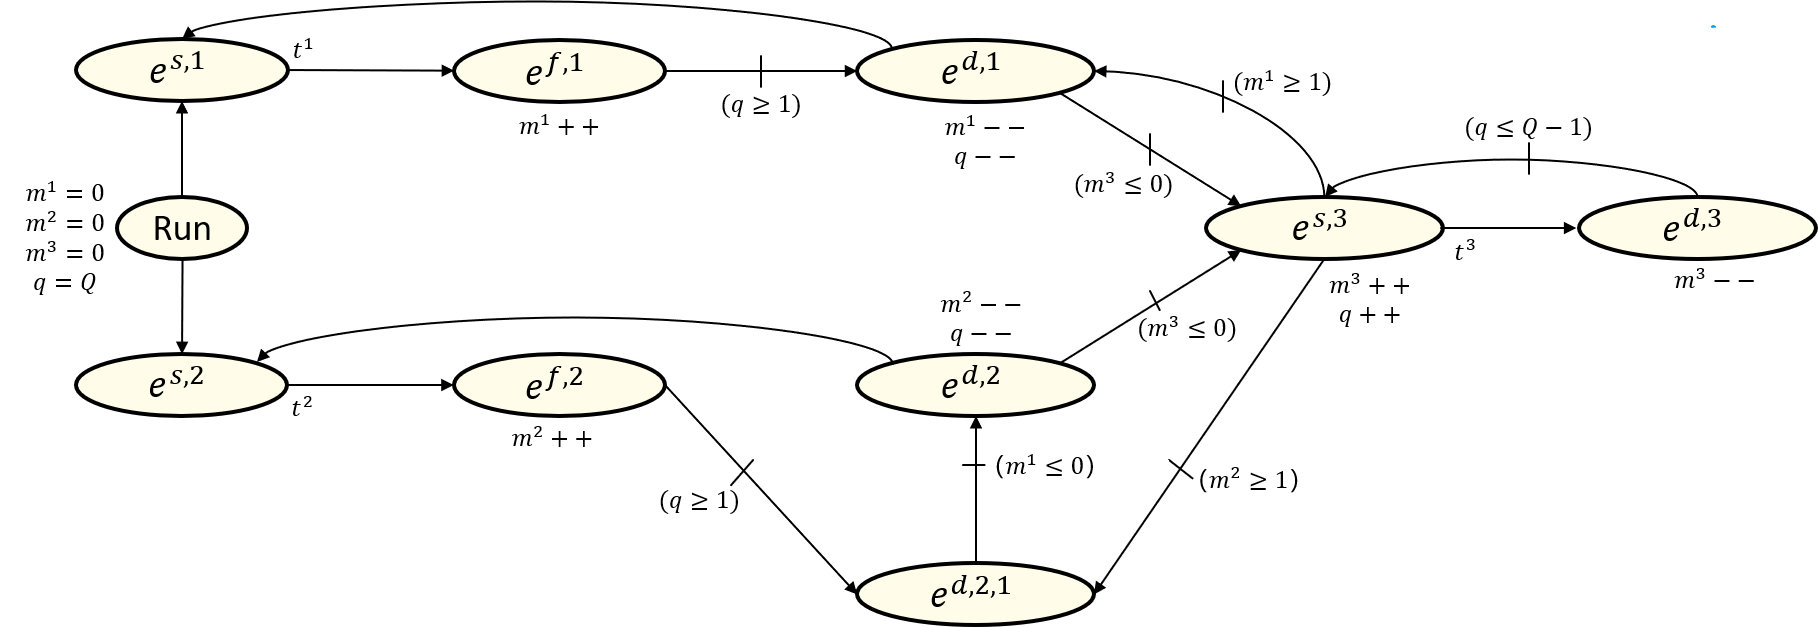
\includegraphics[width=0.6\textwidth]{Figures/ERG_merge.png}
	\caption{ERG of merge queueing system.}
	\label{fig:ERG_merge}
\end{figure}

It can be seen that the model proposed in \cite{chan2008optimization} requires to derive different constraints from each arcs according to the condition on the arc and the state changes of several events. Furthermore, the constraints bound the event execution time from below, which indicate that the event \textit{can} be executed, and the objective function drives the event to be executed as soon as possible. However, the DES model \textit{must} execute the event once the conditions are true, which cannot be guaranteed with the model. To guarantee the equivalence between the MPR  and the simulation implementation, the multiplier of each term of the objective function has to be carefully chosen. Using the model proposed in this work, the objective function can be arbitrary, i.e., any performance indicator can be the objective function.

\subsection{Multiple-server merge}
A multiple-server merge queueing system is shown in Figure \ref{fig:multimerge}. The multiple-server merge queue is a generalization of the system presented in Section 4.1, where the number of parallel servers in station 1, 2 and 3 is equal to $s^1$, $s^2$ and $s^3$, respectively. The state variables are changed accordingly. To describe the state of multiple-server station $j$, two state variables $g^{j}$ and $h^{j}$ are needed to represent the number of idle servers and the number of finished jobs of each the station. The state variable $q$ is used to represent the number of available space in buffer 3. 

\begin{figure}[h]
	\centering
	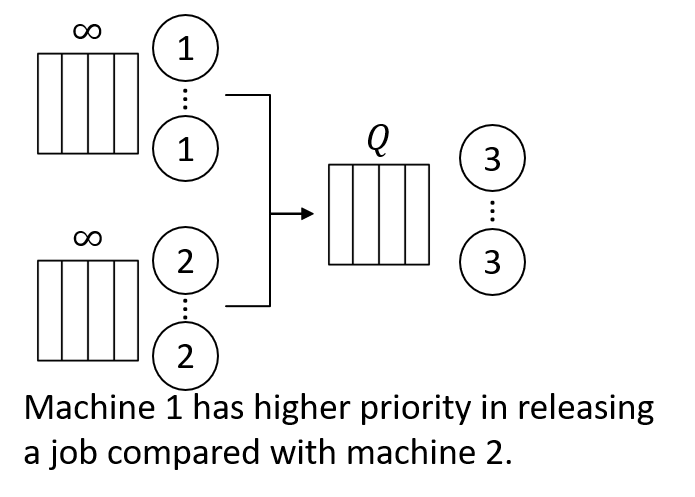
\includegraphics[width=0.4\textwidth]{Figures/multimerge.png}
	\caption{Example: multi-server merge.}
	\label{fig:multimerge}
\end{figure}


The events composing the DES model are shown in Table \ref{tab:multimerge}. The start event of station 1 and 2 is scheduled when there are at least one empty server, and their execution decreases the number of empty servers by one. The scheduling condition of finish event $e^{f,j}$ is the same as $e^{s,j}$, but its execution will increase the number of finished jobs by one. Event $e^{f,j}$ is a multi-execution event with positive delays, an event to count the number of executions of it should be introduced. However, the event $e^{s,j}$ plays that role and the number of executions in the event list is equal to $(s^j-g^j)$. Similarly with single-server system, the departure of station 1 requires that there is at least one finished job in the station and there is at least one space available in buffer 3, but the departure of station 2 also requires that there is no finished job in station 1. The departure of station 1 and 2 will increase the number of empty servers by one, decrease the number of finished jobs by one and decrease the number of available space by one. As for station 3, the start and departure event can be scheduled if there is at least one empty server and one job in buffer 3. Thus, $e^{s,3}$ is used to count the number executions in the event list of $e^{d,3}$. Execution of $e^{s,3}$ will decrease the number of empty server by one and increase the available space in buffer 3 by one.

\begin{table}[h]
	\begin{tabular}{|llllll|}\hline
		Variable&Event & Condition to schedule & Delay&$\beta^{\xi}$& State change\\\hline
		$e^{s,1}$&Start 1 	& $1\le g^1$ & $0$&1& $g^1--$ \\\hline
		$e^{f,1}$&Finish 1 & $1\le g^1$ 	& $t^1$ &$s^1$& $h^1++$\\\hline 
		$e^{d,1}$&Depart 1& $1\le h^1 \&\  q\ge 1$&$0$ &1 & $g^1++,h^1--,\ q--$\\\hline
		$e^{s,2}$&Start 2 	& $1\le g^2$ & $0$ &1& $g^2--$ \\	\hline
		$e^{f,2}$&Finish 2 & $1\le g^2$ 	& $t^2$ &$s^2$ & $h^2++$\\\hline
		$e^{d,2}$&Depart 2& $1\le h^2\ \&\ q\ge 1\ \&$&$0$  &1&  $g^2++,h^2--,\ q--$\\
		&&$\ h^1\le 0 $ & &&\\\hline
		$e^{s,3}$& Start 3 & $1\le g^3\ \&\ q\le Q-1$&$0$  &1& $g^3--,\ q++$\\\hline
		$e^{d,3}$& Depart 3 & $1\le g^3\ \&\ q\le Q-1$ & $t^3$  &$s^3$& $g^3++$\\\hline
	\end{tabular}
	\caption{Events to simulate a multi-server merge queueing system.}
	\label{tab:multimerge}
\end{table}

\newpage
\newpage

\section{Draft}
MP model of single server merge model:
\begin{eqnarray}
\min{\sum_{k}\mathcal{E}_k}\\
e^{(\xi,j),1}_i - \mathcal{E}_{k}\ge M(w^{\xi,j}_{i,k}-1)&&\xi\in\{s,f,d\}, j\in\{1,2,3\},\forall i,k \\
\mathcal{E}_{k} - e^{(\xi,j),1}_i\ge M(w^{\xi,j}_{i,k}-1)&&\xi\in\{s,f,d\}, j\in\{1,2,3\},\forall i,k \\
\sum_{k} w^{\xi,j}_{i,k} =1&& \forall\ \xi\in\{s,f,d\}, j\in\{1,2,3\},i\\
\sum_{(\xi,j),i} w^{\xi,j}_{i,k} =1&& \forall\ k\\
\sum_{k} kw^{\xi,j}_{i+1,k} - \sum_{k} kw^{\xi,j}_{i,k} \ge 1&& \forall\  \xi\in\{s,f,d\}, j\in\{1,2,3\},i\\
e^{s,j,1}_{i} - e^{s,j,0}_{i} \ge 0 && j =1,2,3, \forall \ i\\
e^{f,j,1}_{i} - e^{f,j,0}_{i} \ge t^j_{i}&& j =1,2, \forall \ i\\
e^{d,j,1}_{i} - e^{d,j,0}_{i} \ge 0 && j =1,2, \forall \ i\\
e^{d,3,1}_{i} - e^{d,3,0}_{i} \ge t^3_{i}&&\forall \ i \\
e^{\xi,j,0}_i-\mathcal{E}_{k} \ge M(x^{\xi,j}_{i,k}-1)&& \forall\ \xi\in\{s,f,d\},j=1,2,3,k,i\\
\mathcal{E}_{k} -e^{\xi,j,0}_i\ge M(x^{\xi,j}_{i,k}-1)&& \forall\ \xi\in\{s,f,d\},j=1,2,3,k,i\\
m^j_k=m^j_{k-1} + \sum_{i=1}^{N^{j}} (w^{s,j}_{i,k}  + w^{f,j}_{i,k} - 2w^{d,j}_{i,k})&& j=1,2, \forall\ k\\
m^3_k=m^3_{k-1} + \sum_{i=1}^{N^{3}} (w^{s,3}_{i,k} - w^{d,3}_{i,k})&&\forall\ k\\
q_k = q_{k-1} + \sum_{i=1}^{N^{3}} w^{s,3}_{i,k} - \sum_{i=1}^{N^{1}} w^{d,1}_{i,k} - \sum_{i=1}^{N^{2}} w^{d,2}_{i,k}\\
m^j_k \ge M(z^{s,j}_{k}-1)&& j=1,2,3, \forall \ k\\
1- m^j_k \ge M(z^{f,j}_{k}-1)&& j=1,2, \forall \ k\\
m^j_k - 1 \ge M(z^{f,j}_{k}-1)&& j=1,2, \forall \ k\\
m^j_k - 2 \ge M(z^{d,j}_{k}-1)&& j=1,2, \forall \ k\\
q_k - 1 \ge M(z^{d,j}_{k}-1)&&  j=1,2, \forall \ k\\
1 - m^1_k \ge M(z^{d,2}_{k}-1)&& \forall\ k\\
m^3_k - 1 \ge M(z^{d,3}_{k}-1)&& \forall \ k\\
(Q-1) - q_k \ge M(z^{s,3}_{k}-1)&& \forall\ k\\
\sum_{k} x^{\xi,j}_{i,k} =1&& \forall\ \xi\in\{s,f,d\}, j=1,2,3, \forall\ i,k\\
\sum_{i=1}^{N^{j}}x^{\xi,j}_{i,k} \le z^{\xi,j}_{k}&& \forall\ \xi\in\{s,f,d\}, j=1,2,3, k\\
\sum_{k} kx^{\xi,j}_{i+1,k} - \sum_{k} kx^{\xi,j}_{i,k} \ge 0 && \forall\ \xi\in\{s,f,d\}, j=1,2,3, i
\end{eqnarray}


\section{Resource allocation problem of queueing systems}
\subsection{Mathematical programming representation of simulation model}
We study only the system that the occurrence of an event will lead to the increment or decrement of one unit of the state variables. A simulation model is called a \textit{natural} simulator if the following assumptions all hold:
\begin{enumerate}
		\item An event $e^{\xi}$ can be triggered if the state variables $\mathbf{s}$ satisfy specific conditions \textit{at that time}, regardless of the history of the state or event occurrence, and the condition is not changed along time, i.e., condition is static. It could be possible to define more state variables in case of history dependence and variant triggering conditions.
		\item Natural triggering relationship: if and only if $e^{\xi}$ is an $s$-increment event, $e^{\xi}$ triggers an $s$-decrement event, vice versa.
		\item Natural triggering condition: the condition for triggering an $e^{\xi}$ is that each state variable $s$ must within its predefined domain, i.e., $\mathbf{l} \le\mathbf{s}\le \mathbf{u}$, regardless of event type $\xi$.
		\item For all $e^{\xi}$, the number of execution $N^{\xi}$ is known before simulation, and the simulation terminate when all types of events have been triggered for that number.
\end{enumerate}

Assumptions for a variable $x$ to be resource-type:
\begin{enumerate}
	\item For all $e^{\xi}$, $\mathbf{u}$ is monotonically increasing on $x$, and $\mathbf{l}$ is monotonically decreasing on $x$.
	%\item The condition for triggering an $e^{\xi}$ is in the form of \textit{range}, i.e., $\mathbf{l}^{\xi} \le\mathbf{s}\le \mathbf^{u}^{\xi}$.
	%\item For all $e^{\xi}$, $\mathbf^{u}^{\xi}$ is monotonically increasing on $x$, and $\mathbf{l}^{\xi}$ is monotonically decreasing on $x$.
\end{enumerate}

Formulate the MP model of simulation:

\begin{table}[h]
	\begin{tabular}{ll}
		\hline
		$e^{\xi}_{i}\ge 0$ & time of the $i$-th occurrence of event $e^{\xi}$.\\
		$\tau^{s+}_{l}\ge 0$ & time of the  $l$-th occurrence of events that increments state variable $s$.\\
		$\tau^{s-}_{l}\ge 0$ &   time of the  $l$-th occurrence of events that decrements state variable $s.$\\
		%$c^{\xi,s}_{l}$& the occurring time $l$-th candidate event to trigger event $e^{\xi}$  respect to the condition of state variable $s$.\\		
		$x^{\xi,s+}_{i,l}\in\{0,1\}$& equal to 1 if $e^{\xi}_{i}$ is the $l$-th increment of $s$.\\
		$x^{\xi,s-}_{i,l}\in\{0,1\}$& equal to 1 if $e^{\xi}_{i}$ is the $l$-th decrement of $s$.\\\hline
		%$y^{\xi,s}_{i,l}\in\{0,1\}$ & equal to 1 if the $l$-th candidate event $c^{\xi,s}_{l}$ triggers $e^{\xi}_{i}$.
	\end{tabular}
\end{table} 


The MP model of simulation is
\begin{eqnarray}
&\min\{\sum_{\xi,i} e^{\xi}_{i}\}&\\
&s.t.&\\
&\tau^{s+}_{l} - \tau^{s-}_{l+s_0-u_s} \ge 0& \forall\ s \\
&\tau^{s-}_{l} - \tau^{s+}_{l-s_0+l_s} \ge 0& \forall\ s \\
&\tau^{s+}_{l} - e^{\xi}_{i} \ge M(x^{\xi,s+}_{i,l}-1)& \forall\ s\ and\ e^{\xi}\ with\ increment\ of\ s\\
&\tau^{s-}_{l} - e^{\xi}_{i} \ge M(x^{\xi,s-}_{i,l}-1)& \forall\ s\ and\ e^{\xi}\ with\ decrement\ of\ s\\
&e^{\xi}_{i} - \tau^{s+}_{l} \ge M(x^{\xi,s+}_{i,l}-1) & \forall\ s\ and\ e^{\xi}\ with\ increment\ of\ s\\
&e^{\xi}_{i} - \tau^{s-}_{l} \ge M(x^{\xi,s-}_{i,l}-1) & \forall\ s\ and\ e^{\xi}\ with\ decrement\ of\ s\\
&\sum_{\xi,i} x^{\xi,s+}_{i,l} =1& \forall\ s,l\\
&\sum_{\xi,i} x^{\xi,s-}_{i,l} =1& \forall\ s,l\\
&\sum_{s,l} x^{\xi,s+}_{i,l} =1& \forall\ \xi,i\\
&\sum_{s,l} x^{\xi,s-}_{i,l} =1& \forall\ \xi,i\\
\end{eqnarray}


\newpage
\subsection{Mathematical programming representation of simulation model - V2}

Revise event-based simulation algorithm.

\begin{figure}[h]
	\centering
	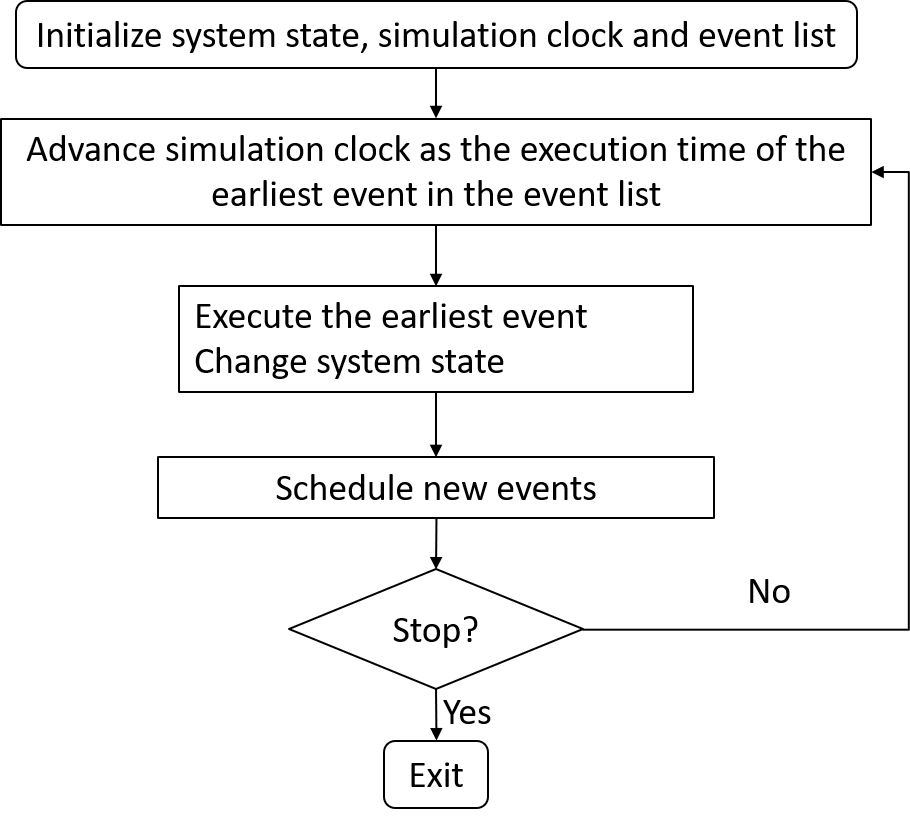
\includegraphics[width=0.6\textwidth]{Figures/EventSimAlgo.png}
	\caption{Event-based simulation algorithm.}
	\label{fig:EventSimAlgo}
\end{figure}

An equivalent mathematical programming model exists if the following assumptions are satisfied:
\begin{enumerate}
	\item State variables are integer.
	\item For all event $e^{\xi}$, the \textit{scheduling conditions} are in the form of $a^{\xi}_s\le s \le c^{\xi}_s$ combined with logic operator ``AND", where $s$ is a state variable, and $a^{\xi}_s$ and $c^{\xi}_s$ are lower and upper bounds.
	\item The scheduling conditions is independent of the history and not changed along time. (It could be possible to define more state variables in case of history dependence and time-variant scheduling conditions.)
	\item An event execution of $e^{\xi}$ leads to integer increment or decrement equal to $\Delta^{\xi}_s$ of certain state variables $s$, and $\Delta^{\xi}_s$ is not changed along time.
	\item The delay between scheduling and execution time of an event $e^{\xi}$, denoted by $t^{\xi}$, is random variate. They can be generated independently from the simulation run. (\textit{This point is different from ERG. In ERG, the delay is dependent on the edge, i.e, a couple of events, but I consider delay dependent on a single event.})
	\item For all events $e^{\xi}$, the number of executions $I^{\xi}$ is known before simulation.
\end{enumerate}

\begin{table}[h]
	\begin{tabular}{ll}
		$e^{\xi}$ & event of type $\xi$\\
		$s$& state variable\\
		$S$& set of all state variables\\
		$S^{\xi}$  & set of state variables whose value is conditioned for scheduling event $e^{\xi}$.\\
		$\Theta^{\xi+}$ & the set of state variables that event $e^{\xi}$ will increase its value.\\
		$\Theta^{\xi-}$ & the set of state variables that event $e^{\xi}$ will decrease its value.\\
		$\Theta^{\xi}$ & $\Theta^{\xi+}\cap\Theta^{\xi-}$\\
		$E^{s+}$ & set of events whose execution increases the value of state variable $s$.\\
		$E^{s-}$  & set of events whose execution decreases the value of state variable $s$.\\
		$\Delta^{\xi}_s$ & increment or decrement of state variable $s$ when event $e^{\xi}$ is executed.\\
		$I^{\xi}$ & total number of executions of event $e^{\xi}$\\
		$L^{s+}$& total number of  times that state variable $s$ is increased.\\
		$L^{s-}$ & total number of  times that state variable $s$ is decreased.\\
		$t^{\xi}$ & delay between scheduling and execution of event $e^{\xi}$.\\
		$t^{\xi}_i$ & delay between $i$-th scheduling and its execution of event $e^{\xi}$.\\
	\end{tabular}
\caption{Notations}
\end{table}


\textbf{Preparation} Event $e^{\xi}$ is expanded into a series of events $e^{\xi,0}$, $e^{\xi,1}$, ..., $e^{\xi,\Delta^{\xi}}$, where $\Delta^{\xi}$ is equal to the maximum among $\Delta^{\xi}_s$ for all $s\in \Theta^{\xi}$. The expansion is conducted as follows. First, event $e^{\xi,0}$ is executed as soon as all the scheduling conditions are satisfied, and the state variables $s\in \Theta^{\xi}$ are not changed. Then, event $e^{\xi,1}$ is executed after $t^{\xi}$ time unit after an execution of $e^{\xi,0}$. For all $s\in \Theta^{\xi}$, if $\Delta^{\xi}_s\ge \delta$,  $e^{\xi,\delta}$ will increase or decrease $s$ by one, for all $\delta=1,...,\Delta^{\xi}$. The $i$-th execution of event $e^{\xi,\delta}$ for $\delta=1,...,\Delta^{\xi}$ are simultaneous.



\begin{table}[h]
	\begin{tabular}{ll}
		$e^{\xi,\delta}_i\ge 0$ 	& time of $i$-th execution of event $e^{\xi,\delta}$\\
		$\tau^{s+}_{l}\ge 0$ 			& time when state variable $s$ is increased for the $l$-th time.  \\
		$\tau^{s-}_{l}\ge 0$ 			& time when state variable $s$ is decreased for the $l$-th time. \\
		$x^{\xi}_{i,i^{'}}\in \{0,1\}$ 	& equal to 1 if the $i^{'}$ execution of event $e^{\xi}$ is the $i$-th scheduled one. \\
		$y^{\xi,\delta,s+}_{i,l}\in \{0,1\}$ & equal to 1 if the $i$-th execution of event $e^{\xi}$ is the $l$-th time that state variable $s$ in increased.\\
		$y^{\xi,\delta,s-}_{i,l}\in \{0,1\}$ &equal to 1 if the $i$-th execution of event $e^{\xi}$ is the $l$-th time that state variable $s$ in decreased.\\
		$z^{\xi,s+}_{i,l}\in \{0,1\}$ & equal to 1 if the $i$-th scheduling of event $e^{\xi}$ is later than $\tau^{s+}_{l}$.\\
	\end{tabular}
\caption{Decision variables}
\end{table}


\textbf{Constraints (A)} The constraints below imply that event $e^{\xi,1}$ is scheduled to execute with a delay $t^{\xi}$, after an execution of $e^{\xi,0}$. 
\begin{eqnarray}
e^{\xi,1}_{i^{'}} - e^{\xi,0}_{i} \ge t^{\xi}_{i} +M(x^{\xi}_{i,i^{'}}-1) && \forall \xi, i, i ^{'}=1,...,I^{\xi}\label{eq::A1}
\end{eqnarray}

It should be noticed that, if multiple executions of the same event $e^{\xi}$ are allow to exist in the future event list simultaneously, the execution of $e^{\xi,1}$ scheduled by the $i$-th execution of $e^{\xi,0}$ may be not the $i$-th execution of $e^{\xi,1}$. Thus, binary variables $x^{\xi}_{i,i^{'}}$ are introduced, and it is equal to one if the $i^{'}$ execution of event $e^{\xi,1}$ is scheduled by the $i$-th execution of event $e^{\xi,0}$. Since each execution of $e^{\xi,0}$ can schedule one and only one execution of $e^{\xi,1}$, the following constraints should also be satisfied:
\begin{eqnarray}
\sum_{i=1}^{N^{\xi}} x^{\xi}_{i,i^{'}} = 1&& \forall\ \xi, i^{'}=1,...,I^{\xi}\\
\sum_{i^{'}=1}^{N^{\xi}} x^{\xi}_{i,i^{'}} = 1 && \forall\ \xi,i=1,...,I^{\xi}
\end{eqnarray}

If up to $\alpha^{\xi}$ multiple executions of event $e^{\xi}$ are allowed, the following constraints can be added:

\begin{eqnarray}
e^{\xi,0}_{i} - e^{\xi,1}_{i-\alpha^{\xi}} \ge 0 && \forall\ \xi,\ i=\alpha^{\xi}+1,...,I^{\xi} \\
\sum_{i^{'}=i+\alpha^{\xi}}^{I^{\xi}} x^{\xi}_{i,i^{'}}=0&& \forall\ \xi,\ i=1,...,I^{\xi}-\alpha^{\xi}\\
\sum_{i=1}^{i^{'}-\alpha^{\xi}} x^{\xi}_{i,i^{'}}=0&&\forall\ \xi,\ i^{'}=\alpha^{\xi}+1, ..., I^{\xi}
\end{eqnarray}

If $\alpha^{\xi}$ is equal to one, the constraints (A) are reduced to:
\begin{eqnarray}
e^{\xi,1}_{i} - e^{\xi,0}_{i} \ge t^{\xi}_{i} && \forall \xi, i=1,...,I^{\xi}\\
e^{\xi,0}_{i} - e^{\xi,1}_{i-1} \ge 0&& \forall\ \xi,\ i=2,...,I^{\xi} 
\end{eqnarray}

\textbf{Constraints (B)} Binding $e^{\xi,\delta}_i$ and $\tau^{s+}_l,\ \tau^{s-}_l$:
\begin{eqnarray}
\tau^{s+}_l - e^{\xi,\delta}_i \ge M(y^{\xi,\delta,s+}_{i,l}-1)&&\forall\ s\in S,e^{\xi}\in E^{s+},\delta=1,..,\Delta^{\xi}_s,i=1,..,I^{\xi},l=1,..,L^{s+} \\
e^{\xi,\delta}_i - \tau^{s+}_l \ge M(y^{\xi,\delta,s+}_{i,l}-1)&&\forall\ s\in S,e^{\xi}\in E^{s+},\delta=1,..,\Delta^{\xi}_s,i=1,..,I^{\xi},l=1,..,L^{s+}\\
\tau^{s-}_l - e^{\xi,\delta}_i \ge M(y^{\xi,\delta,s-}_{i,l}-1)&&\forall\ s\in S,e^{\xi}\in E^{s-},\delta=1,..,\Delta^{\xi}_s,i=1,..,I^{\xi},l=1,..,L^{s-}\\
e^{\xi,\delta}_i - \tau^{s-}_l \ge M(y^{\xi,\delta,s-}_{i,l}-1)&&\forall\ s\in S,e^{\xi}\in E^{s-},\delta=1,..,\Delta^{\xi}_s,i=1,..,I^{\xi},l=1,..,L^{s-}\\
\sum_{\begin{subarray}{c} \xi:e^{\xi}\in E^{s+} \\ i=1,...,I^{\xi}\\\Delta=1,..., \Delta^{\xi}_s\end{subarray}} y^{\xi,\delta,s+}_{i,l}=1&& \forall\ s\in S,l=1,...,L^{s+}\\
\sum_{l=1,...,L^{s+}} y^{\xi,\delta,s+}_{i,l}=1&&\forall\ \xi,s\in \Theta^{\xi+},i=1,...,I^{\xi},\delta=1,...,\Delta^{\xi}_{s}\\
\sum_{\begin{subarray}{c} \xi:e^{\xi}\in E^{s-} \\ i=1,...,I^{\xi}\\\Delta=1,..., \Delta^{\xi}_s\end{subarray}} y^{\xi,\delta,s-}_{i,l}=1&& \forall\ s\in S,l=1,...,L^{s-}\\
\sum_{l=1,...,L^{s-}} y^{\xi,\delta,s-}_{i,l}=1&&\forall\ \xi, s\in \Theta^{\xi-}, i=1,...,I^{\xi},\delta=1,...,\Delta^{\xi}_{s}\\
\end{eqnarray}

Binary variables $y^{\xi,\delta,s+}_{i,l}\in \{0,1\}$ are equal to one if the $i$-th execution of event $e^{\xi,\delta}$ is the $l$-th time that state variable $s$ in increased. Since events $e^{\xi,1},...,e^{\xi,\Delta^{\xi}_s}$ are expanded from one event $e^{\xi}$, and they are executed simultaneously, the following constraints are also added:
\begin{eqnarray}
e^{\xi,\delta}_i = e^{\xi,1}_i && \forall\ \xi,\ i=1,...,I^{\xi}, \delta=1,...,\Delta^{\xi}\\
y^{\xi,\delta,s+}_{i,l+\delta-1} = y^{\xi,1,s+}_{i,l} &&\forall\ \xi,\ s\in\Theta^{\xi+},\ \delta=1,...,\Delta^{\xi}_s,\ i=1,...,I^{\xi}, \ l=1,...,L^{s+}-\Delta^{\xi}_s+1\\
y^{\xi,\delta,s-}_{i,l+\delta-1} = y^{\xi,1,s-}_{i,l} &&\forall\ \xi,\ s\in\Theta^{\xi-},\ \delta=1,...,\Delta^{\xi}_s,\ i=1,...,I^{\xi}, \ l=1,...,L^{s-}-\Delta^{\xi}_s+1
\end{eqnarray}


\textbf{Constraints (C)} To trigger event $e^{\xi,0}$, the conditions $b^{\xi}_s\le s\le c^{\xi}_s$ for all state variable $s\in S^{\xi}$ should be satisfied. $s\in S^{\xi}$ can be categorized into one of the following three situations:
\begin{itemize}
	\item event $e^{\xi}$ does not change the value of $s$, i.e., $s\notin \Theta^{\xi}$.
	\item event $e^{\xi}$ increases the value of $s$, i.e., $s\in \Theta^{\xi+}$. 
	\item event $e^{\xi}$ decreases the value of $s$, i.e., $s\in \Theta^{\xi-}$. 
\end{itemize}

If event $e^{\xi}$ does not change the value of $s$, or if it is executed after being scheduled with positive delay, i.e., $s\notin \Theta^{\xi}$ or $t^{\xi}>0$, the following constraints are applied:
\begin{eqnarray}
e^{\xi,0}_{i} - \tau_{l}^{s+} \le Mz^{\xi,s+}_{i,l} & \forall\ \xi,i=1,...,I^{\xi},\ s\in S^{\xi}, l=1,....,L^{s+}\\
e^{\xi,0}_{i} - \tau_{l}^{s-} \le Mz^{\xi,s-}_{i,l} & \forall\ \xi,\ i=1,...,I^{\xi},\ s\in S^{\xi}, l=1,....,L^{s-}\\
e^{\xi,0}_{i} - \tau_{l}^{s-} \ge -M\hat{z}^{\xi,s-}_{i,l}& \forall\ \xi,\ i=1,...,I^{\xi},\ s\in S^{\xi}, l=1,....,L^{s-}\\
e^{\xi,0}_{i} - \tau_{l}^{s+} \ge -M\hat{z}^{\xi,s+}_{i,l}& \forall\ \xi,\ i=1,...,I^{\xi},\ s\in S^{\xi}, l=1,....,L^{s+}\\
%e^{\xi,0}_{i} - \tau_{s_0+l-b^{\xi}_{s}}^{s-} \ge -M\hat{z}^{\xi,s-}_{i,l}& \forall\ \xi,\ i=1,...,I^{\xi},\ s\in S^{\xi}, l=1,....,L^{s-}??\\
%e^{\xi,0}_{i} - \tau_{-s_0+l+a^{\xi}_{s}}^{s+} \ge -M\hat{z}^{\xi,s+}_{i,l}& \forall\ \xi,\ i=1,...,I^{\xi},\ s\in S^{\xi}, l=1,....,L^{s+}??\\
z^{\xi,s+}_{i,l}+\hat{z}^{\xi,s-}_{i,s_0+l-b^{\xi}_{s}}\le 1&??\\
z^{\xi,s-}_{i,l}+\hat{z}^{\xi,s+}_{i,-s_0+l+a^{\xi}_{s}}\le 1&??\\
%z^{\xi,s+}_{i,l}+\hat{z}^{\xi,s-}_{i,l}\le 1&??\\
%z^{\xi,s-}_{i,l}+\hat{z}^{\xi,s+}_{i,l}\le 1&??
\end{eqnarray}

\begin{eqnarray}
e^{\xi,0}_{i} - \tau_{l}^{s+} \ge M(z^{\xi,s+}_{i,l}-1) & \forall\ \xi,i=1,...,I^{\xi},\ s\in S^{\xi}, l=1,....,L^{s+}\\
\tau_{l}^{s+} - e^{\xi,0}_{i} > -Mz^{\xi,s+}_{i,l}& \forall\ \xi,\ i=1,...,I^{\xi},\ s\in S^{\xi}, l=1,....,L^{s+}\\
e^{\xi,0}_{i} - \tau_{l}^{s-} \ge M(z^{\xi,s-}_{i,l}-1) & \forall\ \xi,\ i=1,...,I^{\xi},\ s\in S^{\xi}, l=1,....,L^{s-}\\
\tau_{l}^{s-} - e^{\xi,0}_{i} > -Mz^{\xi,s-}_{i,l}& \forall\ \xi,\ i=1,...,I^{\xi},\ s\in S^{\xi}, l=1,....,L^{s-}\\
\end{eqnarray}







If $e^{\xi,0}_{i}$ is executed after $\tau_{l}^{s+}$($\tau_{l}^{s-}$), $z^{\xi,s+}_{i,l}$($z^{\xi,s-}_{i,l}$) is equal to one. If $e^{\xi,0}_{i}$ is executed before $\tau_{l}^{s+}$($\tau_{l}^{s-}$), $\hat{z}^{\xi,s+}_{i,l}$($\hat{z}^{\xi,s-}_{i,l}$) is equal to one.


If event $e^{\xi}$ increases the value of $s$, and it is executed immediately when scheduled, i.e., $s\in \Theta^{\xi+}$ and $t^{\xi}=0$, the following constraint should be applied:
\begin{eqnarray}
e^{\xi,0} - \tau^{s-}_{s_0+l-1-b} \ge M(y^{\xi,1,s+}_{i,l}-1)\\
e^{\xi,0} - \tau^{s-}_{s_0+l-1-a} \le M(1-y^{\xi,1,s+}_{i,l})
\end{eqnarray}

If event $e^{\xi}$ decreases the value of $s$, and it is executed immediately when scheduled, i.e., $s\in \Theta^{\xi-}$ and $t^{\xi}=0$, the following constraint should be applied:
\begin{eqnarray}
e^{\xi,0} - \tau^{s+}_{-s_0+l-1+a} \ge M(y^{\xi,1,s-}_{i,l}-1)\\
e^{\xi,0} - \tau^{s+}_{-s_0+l-1+b} \le M(1-y^{\xi,1,s-}_{i,l})
\end{eqnarray}



\newpage
\subsection{Mathematical programming representation of simulation model - V3}
Event-scheduling algorithm for DES. 

\begin{figure}[h]
	\centering
	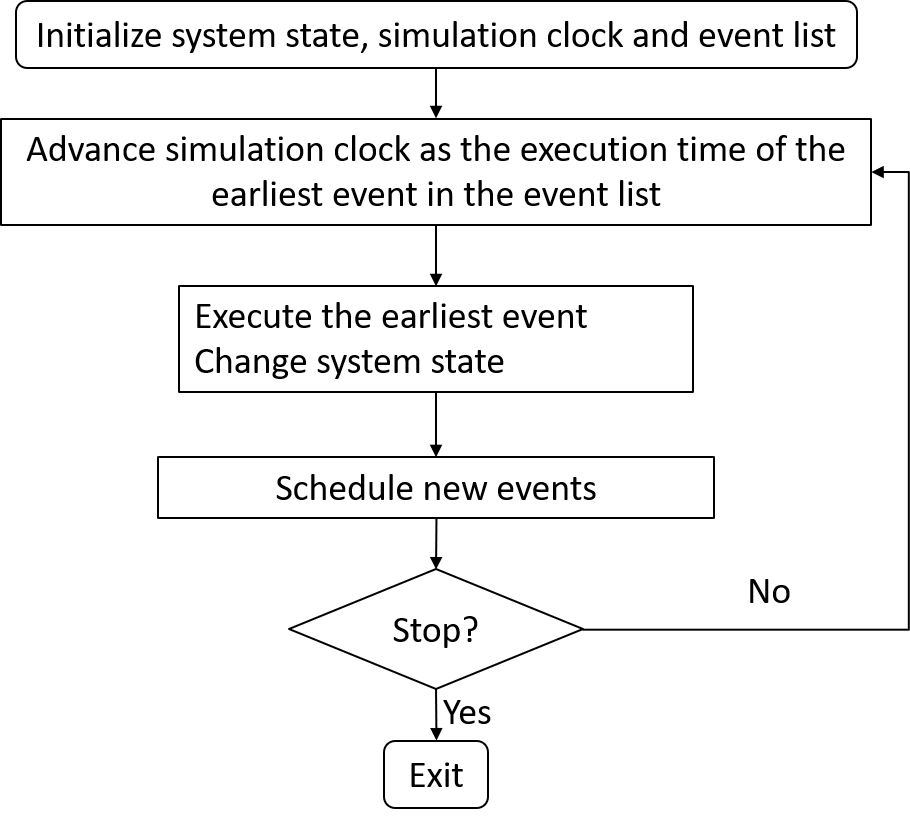
\includegraphics[width=0.8\textwidth]{Figures/EventSimAlgo.png}
	\caption{Event-based simulation algorithm.}
\end{figure}


An equivalent mathematical programming model exists if the following assumptions are satisfied:
\begin{enumerate}
	% \item State variables are integer.
	\item For all event $e^{\xi}$, the \textit{scheduling conditions} are in the form of $b^{\xi}_s\le s \le c^{\xi}_s$ combined with logic operator ``AND", where $s$ is a state variable, and $b^{\xi}_s$ and $c^{\xi}_s$ are lower and upper bounds.
	\item The scheduling conditions is independent of the history and not changed along time. (It could be possible to define more state variables in case of history dependence and time-variant scheduling conditions.)
	\item An event execution of $e^{\xi}$ leads to (integer) increment or decrement equal to $\Delta^{\xi}_s$ of certain state variables $s$, and $\Delta^{\xi}_s$ is not changed along time. (A direct evaluation can be modeled in this way.)
	\item The delay between scheduling and execution time of an event $e^{\xi}$, denoted by $t^{\xi}$, is random variate. They can be generated independently from the simulation run. (\textit{This point is different from ERG. In ERG, the delay is dependent on the edge, i.e, a couple of events, but I consider delay dependent on a single event.})
	\item For all events $e^{\xi}$, the number of executions $N^{\xi}$ is known before simulation.
\end{enumerate}

\begin{table}[h]
	\begin{tabular}{lll}
		$e^{\xi,0}_{i}\ge 0$ & $i$=1,...,$I^{\xi}$& the $i$-th scheduling time of event $e^{\xi}$.\\
		$e^{\xi,1}_{i}\ge 0$ & $i$=1,...,$I^{\xi}$& the $i$-th execution time of event $e^{\xi}$.\\
		$\mathcal{E}_k\ge 0$ &$k$=0,...,$K$& time of the $k$-th execution of any events.\\
		$u^s_k\in \mathbb{Z}$ &$k$=0,...,$K$& value of state variable $s$ just after the $k$-th event.\\
		$w^{\xi}_{i,k}\in \{0,1\}$ &$k$=1,...,$K$& binding $e^{\xi,1}_i$ and $\mathcal{E}_k$.\\
		$x^{\xi}_{i,k}\in\{0,1\}$ &$k$=0,...,$K$& equal to one if $\mathcal{E}_k$ schedules $e^{\xi,0}$.\\
		$y^{\xi}_{i,i^{'}}\in\{0,1\}$&& binding $e^{\xi,0}_i$ and $e^{\xi,1}_{i^{'}}$ in case of overtaking.\\
		$z^{\xi}_{k}\in\{0,1\}$ &$k$=0,...,$K$& equal to one if the condition for scheduling $e^{\xi}$ is true right after $\mathcal{E}_k$.\\ 
		$v^{\xi,s,0}_k\in\{0,1\}$ &$k$=0,...,$K$& equal to one if $s_k\le a^{\xi,s}-1$\\
		$v^{\xi,s,1}_k\in\{0,1\}$ &$k$=0,...,$K$& equal to one if $s_k\ge b^{\xi,s}-1$\\
		$r^{\xi}_k\in \mathbb{Z}$ &$k$=0,...,$K$& number of existing parallel executions of $e^{\xi,1}_i$ after $\mathcal{E}_k$ before scheduling.\\
		$n^{\xi}_k\in \mathbb{Z}$ & $k$=0,...,$K$ & number of scheduled executions of $e^{\xi,1}_i$ after $\mathcal{E}_k$ before scheduling.\\
	\end{tabular}
\caption{Notation}
\end{table}

\textbf{Constraints (A):} binding $e^{\xi,1}_i$ and $\mathcal{E}_k$:
\begin{eqnarray}
	e^{\xi,1}_i-\mathcal{E}_k\ge M(w^{\xi}_{i,k}-1) &A1& \forall\ \xi,i,k\\
	\mathcal{E}_k-e^{\xi,1}_i\ge M(w^{\xi}_{i,k}-1) &A2& \forall\ \xi,i,k\\
	\sum_{k} w^{\xi}_{i,k} =1&A3& \forall\ \xi,i\\
	\sum_{\xi,i} w^{\xi}_{i,k} =1&A4& \forall\ k\\
	\sum_{k} kw^{\xi}_{i+1,k} - \sum_{k} kw^{\xi}_{i,k} \ge 1&A5& \forall\ \xi,i
\end{eqnarray}

\textbf{Constraints (B):} binding $e^{\xi,0}_i$ and $e^{\xi,1}_{i^{'}}$, where $\alpha^{\xi}$ is the maximal number of executions existing simultaneously in the event list:
\begin{eqnarray}
e^{\xi,1}_{i^{'}} - e^{\xi,0}_{i} \ge t^{\xi}_{i} +M(y^{\xi}_{i,i^{'}}-1) &B1& \forall \xi, i, i ^{'}=1,...,N^{\xi}\\
e^{\xi,0}_{i} - e^{\xi,1}_{i^{'}}  \ge -t^{\xi}_{i} +M(y^{\xi}_{i,i^{'}}-1) &B2& \forall \xi, i, i ^{'}=1,...,N^{\xi}\\
\sum_{i=1}^{N^{\xi}} y^{\xi}_{i,i^{'}} = 1&B3& \forall\ \xi, i^{'}=1,...,N^{\xi}\\
\sum_{i^{'}=1}^{N^{\xi}} y^{\xi}_{i,i^{'}} = 1 &B4& \forall\ \xi,i=1,...,N^{\xi}\\
%e^{\xi,0}_{i} - e^{\xi,1}_{i-\alpha^{\xi}} \ge 0 && \forall\ \xi,\ i=\alpha^{\xi}+1,...,N^{\xi} \\
\sum_{i^{'}=i+\alpha^{\xi}}^{N^{\xi}} y^{\xi}_{i,i^{'}}=0&B5& \forall\ \xi,\ i=1,...,N^{\xi}-\alpha^{\xi}\\
\sum_{i=1}^{i^{'}-\alpha^{\xi}} y^{\xi}_{i,i^{'}}=0&B6&\forall\ \xi,\ i^{'}=\alpha^{\xi}+1, ..., N^{\xi}
\end{eqnarray}
If $\alpha^{\xi}=1$, variables $y^{\xi}_{i,i^{'}}$ are redundant and constraints (B) are reduced to:
\begin{eqnarray}
e^{\xi,1}_{i} - e^{\xi,0}_{i} = t^{\xi}_{i} &B1& \forall \xi, i=1,...,N^{\xi}
% e^{\xi,0}_{i} - e^{\xi,1}_{i-1} \ge 0 && \forall\ \xi,\ i=2,...,N^{\xi} 
\end{eqnarray}
Number of executions of event $e^{\xi}$ waiting in the event list can be a state variable $n^{\xi}$, and one condition for scheduling an $e^{\xi}$ is $n^{\xi}\le \alpha^{\xi}$. Thus, it can be managed as a generic scheduling condition.

\textbf{Constraints (C):} event $e^{\xi}$ can be scheduled right after $\mathcal{E}_k$ if all state variables $s$ satisfies condition $a^{\xi}_{s}\le s_k\le b^{\xi}_{s}$. 
\begin{eqnarray}
e^{\xi,0}_i-\mathcal{E}_{k} \ge M(x^{\xi}_{i,k}-1)&C1& \forall\ \xi,k,i\\
\mathcal{E}_{k} -e^{\xi,0}_i\ge M(x^{\xi}_{i,k}-1)&C2& \forall\ \xi,k,i\\
\sum_{k} x^{\xi}_{i,k} =1&C3& \forall\ \xi,i\\
b^{\xi,s} - u^s_k \ge M(z^{\xi}_{k}-1)&C4& \forall\ \xi, k,s\\
% - u^s_k \ge U^{s}(z^{\xi}_{k}-1)-b^{\xi,s}z^{\xi}_{k}&C4& \forall\ \xi, k,s\\
 u^s_k - a^{\xi,s} \ge M(z^{\xi}_{k}-1)&C5& \forall\ \xi, k,s\\
%u^s_k  \ge a^{\xi,s}z^{\xi}_{k} -L^{s}(z^{\xi}_{k}-1)&C5& \forall\ \xi, k,s\\
u^s_k -  (b^{\xi,s}+1) \ge M(v^{\xi,s,1}_k-1) &C6& \forall\ \xi,k,s\\
%u^s_k \ge (b^{\xi,s}+1)v^{\xi,s,1}_k -L^s(v^{\xi,s,1}_k-1)&C6& \forall\ \xi,k,s\\
( a^{\xi,s}-1) - u^s_k \ge M(v^{\xi,s,0}_k-1) &C7& \forall\ \xi,k,s\\
% - u^s_k \ge U^s(v^{\xi,s,0}_k-1)-(a^{\xi,s}-1)v^{\xi,s,0}_k &C7& \forall\ \xi,k,s\\
1 - z^{\xi}_{k} \le \sum_{s\in S^{\xi}} v^{\xi,s,0}_k + \sum_{s\in S^{\xi}} v^{\xi,s,1}_k + v^{\xi,r}_k + v^{\xi,N}_k&C8&\forall\ \xi,k\\
\sum_{i=1}^{N^{\xi}}x^{\xi}_{i,k} = z^{\xi}_k&C9&\forall\ \xi,k\\
%X^{\xi}_k  = z^{\xi}_{k}  &C90& \forall\ \xi, k\\
% - r^{\xi}_{k} \le N^{\xi} - n^{\xi}_{k} -R^{\xi}\beta^{\xi}_k&C91&\forall\ \xi, k\\
%N^{\xi} - n^{\xi}_{k} \le R^{\xi} - r^{\xi}_{k} +N^{\xi}\beta^{\xi}_k&C92&\forall\ \xi, k\\
%X^{\xi}_k\ge R^{\xi}(z^{\xi}_k + \beta^{\xi}_k-1) - r^{\xi}_{k}&C93&\forall\ \xi, k\\
%X^{\xi}_k\ge N^{\xi}z^{\xi}_k - N^{\xi}\beta^{\xi}_k - n^{\xi}_{k}&C94&\forall\ \xi, k\\
\sum_{k} kx^{\xi}_{i+1,k} - \sum_{k} kx^{\xi}_{i,k} \ge 1&C10& \forall\ \xi,i
\end{eqnarray}

%If $r^{\xi}_{max}=1$, then constraints C9 to C94 is reduced to 
%\begin{eqnarray}
%\sum_{i=1}^{N^{\xi}}x^{\xi}_{i,k} = z^{\xi}_k&C9&\forall\ \xi,k
%\end{eqnarray}

\textbf{Constraints (D):} evolution of state variables
\begin{eqnarray}
u^{s}_{k} = u^s_{k-1} + \sum_{\xi} \sum_{i=1}^{N^{\xi}} w^{\xi}_{i,k} \Delta^{\xi,s}&D1& \forall\ s,k\\
r^{\xi}_k = r^{\xi}_{k-1} + X^{\xi}_{k-1} - \sum_i w^{\xi}_{i,k} &D2& \forall\ \xi,k\\
R^{\xi} - r^{\xi}_k \ge z^{\xi}_k&D3& \forall\ \xi,k\\
r^{\xi}_k  \ge R^{\xi}v^{\xi,r}_k&D4& \forall\ \xi,k\\
n^{\xi}_k = n^{\xi}_{k-1} + X^{\xi}_{k-1} &D5& \forall\ \xi,k\\
N^{\xi} - n^{\xi}_k \ge z^{\xi}_k&D6&\forall\ \xi,k\\
n^{\xi}_k \ge N^{\xi}v^{\xi,N}_k&D7&\forall\ \xi,k
\end{eqnarray}

\textbf{Constraints (E):} others
\begin{eqnarray}
\mathcal{E}_{0} = 0&E1&\\
\mathcal{E}_{k}-\mathcal{E}_{k-1}\ge 0&E1&\forall\ k
\end{eqnarray}

%Constraints (D): for zero-delay event $e^{\xi}$, $\alpha^{\xi}$ is equal to 1. Thus, $e^{\xi,0}_{i+1}$ can be scheduled after the execution of $e^{\xi,1}_{i}$
%\begin{eqnarray}
%x^{\xi}_{i+1,k}\le \sum_{k^{'}=1}^{k} w^{\xi}_{i,k^{'}} && \forall\ \text{zero-delay event}\ e^{\xi}
%\end{eqnarray}

\textbf{Objective function:} with the constraints above, there is a unique solution in terms of event occurring times (solution of the binary variables could be multiple in case of multiple simultaneous events). Thus, the objective can be any function of event occurring time. I tried minimize/maximize the sum of $\mathcal{E}_k$, and they give the same solution.

\textbf{Conditions for a variable $x$ to be \textit{resource-type} are not valid any more.}
\begin{enumerate}
\item $\forall\ \xi$ and $s$, upper bound $c^{\xi}_s$ is monotonically increasing on $x$.
\item  $\forall\ \xi$ and $s$, lower bound $b^{\xi}_s$ is monotonically decreasing on $x$.
%\item $\forall\ \xi$, maximal number of executions waiting in the event list simultaneously $\alpha^{\xi}$ in monotonically increasing on $x$.
\end{enumerate}

The reason is that increasing $c^{\xi}_s$ or decreasing $b^{\xi}_s$ will tighten constraints C6 and C7. To be simple, we consider $b$ only. 
\begin{eqnarray}
b - u^s_k \ge M(z^{\xi}_{k}-1)&C4-b& \forall\ \xi, k,s\\
u^s_k -  (b+1) \ge M(v^{\xi,s,1}_k-1) &C6-b& \forall\ \xi,k,s
\end{eqnarray}
(when $u=b+1$, event $e^{\xi}$ cannot be scheduled.)

If $b$ is increased to $b+1$:
\begin{eqnarray}
(b+1) - u^s_k \ge M(z^{\xi}_{k}-1)&C4-(b+1)& \forall\ \xi, k,s\\
u^s_k -  (b+2) \ge M(v^{\xi,s,1}_k-1) &C6-(b+1)& \forall\ \xi,k,s
\end{eqnarray}
(when $u=b+1$, event $e^{\xi}$ must be scheduled.)

A group of relaxed constraints are:
\begin{eqnarray}
(b+1) - u^s_k \ge M(z^{\xi}_{k}-1)&C4-(b+1)& \forall\ \xi, k,s\\
u^s_k -  (b+1) \ge M(v^{\xi,s,1}_k-1) &C6-(b)& \forall\ \xi,k,s
\end{eqnarray}
(when $u=b+1$, event $e^{\xi}$ can be scheduled or not.)


Todo: 
\begin{enumerate}
	\item What kind of performance indicators can be used? (Regular function of time, in scheduling area. Weighted sum, maximum. Refer to book on scheduling.)
\end{enumerate}

\newpage

\subsection{Merge}
\begin{figure}[h]
	\centering
	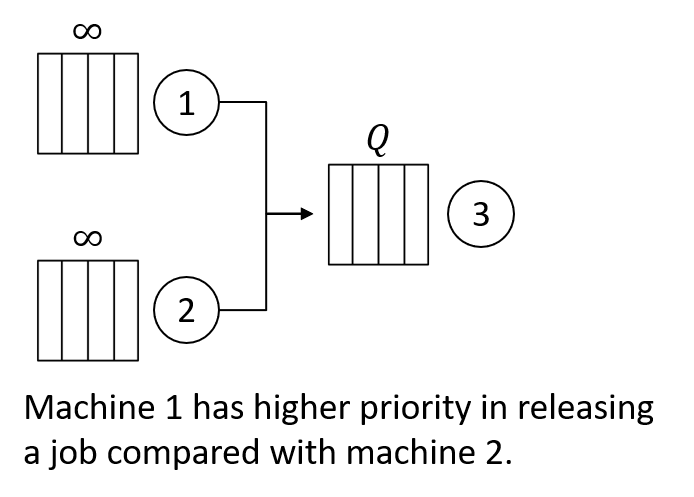
\includegraphics[width=0.9\textwidth]{Figures/merge.png}
	\caption{Example: merge.}
\end{figure}

\begin{table}[h]
	\begin{tabular}{|llllll|}\hline
		Variable&Event & Condition to schedule & Delay&\# executions& State change\\\hline
		$e^{s,1}$&Start m1 	& $m^1\le 0$ & $0$&1& $m^1++$ \\\hline
		$e^{f,1}$&Finish m1 & $1\le m^1\le 1$ 	& $t^1$ &1& $m^1++$\\\hline
		$e^{d,1}$&Depart m1& $m^1\ge2\ AND$&$0$ &1 & $m^1 = m^1-2,\ q--$\\
											&&$ q\ge 1$ &&&\\\hline
		$e^{s,2}$&Start m2 	& $m^2\le 0$ & $0$ &1& $m^2++$ \\	\hline
		$e^{f,2}$&Finish m2 & $1\le m^2\le 1$ 	& $t^2$ &1 & $m^2++$\\\hline
		$e^{d,2}$&Depart m2& $m^2\ge2\ AND$&$0$  &1& $m^2=m^2-2,\ q--$\\
						&&$\ q\ge 1\ AND$&&&\\
						&&$\ m^1\le 1 $ & &&\\\hline
		$e^{s,3}$& Start m3 & $m^3 \le 0\ AND$&$0$  &1& $m^3++,\ q++$\\
						&&$\ q\le Q-1$ & &&\\\hline
		$e^{d,3}$& Depart m3 & $m^3 \ge 1$ & $t^3$  &1& $m^3--$\\\hline
	\end{tabular}
	\caption{Merge-S3M111}
\end{table}

MP model:
\begin{eqnarray}
\min{\sum_{k}\mathcal{E}_k}\\
e^{(\xi,j),1}_i - \mathcal{E}_{k}\ge M(w^{\xi,j}_{i,k}-1)&&\xi\in\{s,f,d\}, j\in\{1,2,3\},\forall i,k \\
\mathcal{E}_{k} - e^{(\xi,j),1}_i\ge M(w^{\xi,j}_{i,k}-1)&&\xi\in\{s,f,d\}, j\in\{1,2,3\},\forall i,k \\
\sum_{k} w^{\xi,j}_{i,k} =1&& \forall\ \xi\in\{s,f,d\}, j\in\{1,2,3\},i\\
\sum_{(\xi,j),i} w^{\xi,j}_{i,k} =1&& \forall\ k\\
\sum_{k} kw^{\xi,j}_{i+1,k} - \sum_{k} kw^{\xi,j}_{i,k} \ge 1&& \forall\  \xi\in\{s,f,d\}, j\in\{1,2,3\},i\\
e^{s,j,1}_{i} - e^{s,j,0}_{i} \ge 0 && j =1,2,3, \forall \ i\\
e^{f,j,1}_{i} - e^{f,j,0}_{i} \ge t^j_{i}&& j =1,2, \forall \ i\\
e^{d,j,1}_{i} - e^{d,j,0}_{i} \ge 0 && j =1,2, \forall \ i\\
e^{d,3,1}_{i} - e^{d,3,0}_{i} \ge t^3_{i}&&\forall \ i \\
e^{\xi,j,0}_i-\mathcal{E}_{k} \ge M(x^{\xi,j}_{i,k}-1)&& \forall\ \xi\in\{s,f,d\},j=1,2,3,k,i\\
\mathcal{E}_{k} -e^{\xi,j,0}_i\ge M(x^{\xi,j}_{i,k}-1)&& \forall\ \xi\in\{s,f,d\},j=1,2,3,k,i\\
m^j_k=m^j_{k-1} + \sum_{i=1}^{N^{j}} (w^{s,j}_{i,k}  + w^{f,j}_{i,k} - 2w^{d,j}_{i,k})&& j=1,2, \forall\ k\\
m^3_k=m^3_{k-1} + \sum_{i=1}^{N^{3}} (w^{s,3}_{i,k} - w^{d,3}_{i,k})&&\forall\ k\\
q_k = q_{k-1} + \sum_{i=1}^{N^{3}} w^{s,3}_{i,k} - \sum_{i=1}^{N^{1}} w^{d,1}_{i,k} - \sum_{i=1}^{N^{2}} w^{d,2}_{i,k}\\
m^j_k \ge M(z^{s,j}_{k}-1)&& j=1,2,3, \forall \ k\\
1- m^j_k \ge M(z^{f,j}_{k}-1)&& j=1,2, \forall \ k\\
m^j_k - 1 \ge M(z^{f,j}_{k}-1)&& j=1,2, \forall \ k\\
m^j_k - 2 \ge M(z^{d,j}_{k}-1)&& j=1,2, \forall \ k\\
q_k - 1 \ge M(z^{d,j}_{k}-1)&&  j=1,2, \forall \ k\\
1 - m^1_k \ge M(z^{d,2}_{k}-1)&& \forall\ k\\
m^3_k - 1 \ge M(z^{d,3}_{k}-1)&& \forall \ k\\
(Q-1) - q_k \ge M(z^{s,3}_{k}-1)&& \forall\ k\\
\sum_{k} x^{\xi,j}_{i,k} =1&& \forall\ \xi\in\{s,f,d\}, j=1,2,3, \forall\ i,k\\
\sum_{i=1}^{N^{j}}x^{\xi,j}_{i,k} \le z^{\xi,j}_{k}&& \forall\ \xi\in\{s,f,d\}, j=1,2,3, k\\
\sum_{k} kx^{\xi,j}_{i+1,k} - \sum_{k} kx^{\xi,j}_{i,k} \ge 0 && \forall\ \xi\in\{s,f,d\}, j=1,2,3, i
\end{eqnarray}

\newpage
\subsection{Merge - 2 machines in station 3}
\begin{table}[h]
	\begin{tabular}{|llll|}\hline
		Variable&Value & Initialization& Description\\\hline
		$e^1$& 0,1,2&  2 &number of empty machines in station 1 \\\hline
		$f^1$&0,1,2	& 0 & number of finished jobs in station 1\\\hline
		$e^2$&0,1&1&number of empty machines in station 2 \\\hline
		$f^2$&0,1&0&number of finished jobs in station 2 \\\hline
		$e^3$&0,1&1&number of empty machines in station 3  \\	\hline
		$q$& 0,...,Q&Q&  number of available spaces in queue\\\hline
	\end{tabular}
	\caption{State variables: Merge-S3M211}
\end{table}


\begin{table}[h]
	\begin{tabular}{|llllll|}\hline
		Variable&Event & Condition to schedule & Delay&\# executions& State change\\\hline
	ai 	$e^{f,1}$&Finish m1 &  $1 \le  e^1 \le 2$	& $t^1$ &2& $f^1++$\\\hline
		$e^{d,1}$&Depart m1& $1\le   f^1  \le 2\ AND$&$0$ &1 & $e^1++,\ f^1--,\ q--$\\
											&&$ 1\le q\le Q$ &&&\\\hline
		$e^{s,2}$&Start m2 	& $1\le e^2\le 1$ & $0$ &1& $e^2--$ \\	\hline
		$e^{f,2}$&Finish m2 & $1\le e^2\le 1$ 	& $t^2$ &1 & $f^2++$\\\hline
		$e^{d,2}$&Depart m2&$1\le f^2 \le 1\ AND$&$0$  &1& $f^2--,e^2++,\ q--$\\
		&&$\ 1\le q\le Q\ AND$&&&\\
		&&$\ 0\le f^1\le 0 $ & &&\\\hline
		$e^{s,3}$& Start m3 & $1\le e^3\le 1\ AND$&$0$  &1& $e^3--,\ q++$\\
		&&$\ 0\le q\le Q-1$ & &&\\\hline
		$e^{d,3}$& Depart m3 & $1 \le e^3\le 1\ AND $ & $t^3$  &1& $e^3++$\\\hline
		&&$\ 0\le q\le Q-1$ & &&\\\hline
	\end{tabular}
	\caption{Events: Merge-S3M211}
\end{table}



\newpage
\subsection{Failure}



\newpage
\subsection{Jobshop}


\subsection{Identifying Resource-type variables}


\section{Gradient-based approximate cut}
\subsection{Gradient estimation}
\subsection{Gradient-based feasibility cut}


\section{Combinatorial cut generation}
\subsection{Combinatorial cut}
\subsection{Heuristic for tightening Exact combinatorial cut}

\section{Feasibility-cut-based algorithm}
The complete algorithm for solving RAP--PC is summarized in Algorithm 1. The resource capacities are initialized to the lower bound. The searching region of RAP--PC--MIP is initialized to $\Bbb{X}$, and the lower and upper bounds of the objective function, $C^L$ and $C^U$, respectively,  are set considering the upper bound and lower bound of the capacity of each resource. Lines 7 to 11 show that approximate cuts are generated and used in the model when infeasible solutions are found. Once a feasible solution is found, the upper bound $C^U$, which is also the incumbent solution, can be updated after comparing the value of the found feasible solution and that of the current incumbent. Then, all the currently used approximate cuts are replaced by exact cuts of the DIS. If there are only exact cuts in RAP--PC--MIP, the solution is the new lower bound $C^L$. The algorithm terminates when the gap between the upper bound and lower bound is within a tolerance or the time limit is exceeded.

\begin{algorithm}[h]
	\label{algo:}
	\caption{MIP--based algorithm.}
	\begin{algorithmic}[1]
		\REQUIRE ~~\\
		Lower bound $\mathbf{a}=[a_1,...,a_J]$ and upper bound $\mathbf{b}=[b_1,...,b_J]$ of resource capacity $\mathbf{x}$, such that $a_j\le x_j\le b_j\ \forall\ j=1,...,J$. \\
		Tolerance of optimality gap $\varepsilon_{opt}$.\\
		Optional input: time limit of the algorithm $T_{lim}$.\\
		\ENSURE ~~\\
		Sample-path global optimal $\mathbf{x}^*$.\\
		\STATE Initialize system with lower bound $\mathbf{x}\leftarrow\mathbf{a}$
		\STATE Initialize incumbent with upper bound $\mathbf{x}^*\leftarrow\mathbf{b}$. 
		\STATE Initialize lower bound of the objective $C^{L}\leftarrow\mathbf{c}^T\mathbf{a}$.
		\STATE Initialize upper bound of the objective $C^{U}\leftarrow\mathbf{c}^T\mathbf{b}$.
		\STATE Add initial constraints which defines $\Bbb{X}$ to the RAP--PC--MIP.
		\WHILE {$C^{U}-C^{L}>\varepsilon_{opt}$ and $T_{lim}$ is not exceeded.}
		\WHILE {There exists at least one violated performance constraint}
		\STATE Generate one approximate cut $CA(\bar{\mathbf{x}},l)$ for each violated constraints $l$ and add all the generated cuts to the RAP--PC--MIP.
		\STATE $\bar{\mathbf{x}}\leftarrow$ solution of the RAP--PC--MIP.
		\STATE Simulate the system of $\bar{\mathbf{x}}$.
		\ENDWHILE
		\STATE Update upper bound and incumbent $C^{U}\leftarrow\mathbf{c}^T\bar{\mathbf{x}},\ \mathbf{x}^*\leftarrow \bar{\mathbf{x}}$ if $\mathbf{c}^T\bar{\mathbf{x}}< C^{U}$.
		\IF {There exist approximate cuts in RAP--PC--MIP}
		\STATE For all the currently used approximate cuts $CA(\bar{\mathbf{x}}^r,l)$, find dominating infeasible solution $\bar{\mathbf{x}}_d(\bar{\mathbf{x}}^r)$ and replace approximate cuts $CA(\bar{\mathbf{x}}^r,l)$ by exact cuts $CE(\bar{\mathbf{x}}_d(\bar{\mathbf{x}}^r),l)$ of the DIS.
		\STATE $\bar{\mathbf{x}}\leftarrow$ solution of the RAP--PC--MIP.
		\STATE Simulate the system of $\bar{\mathbf{x}}$.
		\STATE Update lower bound $C^L\leftarrow \max\{\mathbf{c}^T\bar{\mathbf{x}},\ C^L\}$.
		\ENDIF	
		\ENDWHILE
	\end{algorithmic}
\end{algorithm}


\section{Numerical analysis}

\section{Conclusion}




%Reference
\bibliographystyle{apacite}
\bibliography{RAP}

\end{document}
